% !TeX spellcheck = en_US

\chapter{Infrastructural code generation}
\label{chap: Code generation}
\section{Introduction}
After designing an OBSW model using the OSRA SCM model editor and following the component-based software development approach that comes with it, the OBSW model entities need to be mapped to the infrastructure code. The reference programming model for OSRA, discussed in the previous chapter helps us in progressing towards this goal. But, it is necessary to understand the overall design approach for the generated code and briefly present the abstractions that will be offered to the software supplier. This chapter, deals with these things in detail. Similar efforts from the Artemis JU CHESS project \cite{EvoRAVCodeAr}, provide the perfect base for discussions in this chapter of the Master thesis.   

\section{User model entities in the Platform Independent Model (PIM) phase}
A detailed description of all the modeling entities that the software architect can use, can be found in the specification of the metamodel for the OSRA component model \cite{SpecMetamodel}. However a brief description of them is noteworthy here:
 
\begin{description}
\item [Datatypes] The software architect can create a set of project-specific data types and constants using the \texttt{Data Types} language unit of the \texttt{CommonTypes} metamodel and the language unit is designed to provide the software architect an expressive power comparable to the languages with strong types (e.g. Ada).\cite{SpecMetamodel}. The supported type definitions are boolean types, integer types, float types, enumeration types, fixed point types, array types, structured types, string types, union types, alias types, opaque types, external types and unconstrained types. Some of these data type definitions are obvious for readers with programming skills in typed languages such as Ada, C or C++. 

\item [Interface] An interface is a specification of coherent set of services and it represents the definition of a contract. An interface is defined independently of the entities implementing it (e.g. Component type). An interface may enlist declaration of operations, which are the functional services that shall be offered by the entities implementing it. The services include a name, set of ordered parameters and one or more exceptions that they might throw when things go wrong during the handling of the service. Parameters are typed with one of the types mentioned above and have a mode (\texttt{in, out} or \texttt{inout}). A component type may expose one or more interfaces and the same interface can be exposed by different component types. An interface may also contain the declaration of one or more interface attributes, which are the parameters that are accessible via the interface implementations.

\item [Component type] A component type is an entity which specifies the external interfaces of a software component and are defined in isolation and are used to declare relationships with the other components and system in general. It conforms to the principle of encapsulation and as a consequence, all the interactions with other components are performed exclusively via its explicitly declared interface. A component type usually encompasses:
\begin{itemize}
\item A list of provided interface ports
\item A list of required interface ports
\item A list of dataset emitter ports 
\item A list of dataset receiver ports
\item A list of event emitter ports
\item A list of event receiver ports 
\end{itemize}

\item [Component implementation] It is an entity that represents a concrete realization of a component type. It is functionally identical to the component type except that the source code is added to the component implementation and may also define number of component implementation attributes

\item [Component instance] It is an instantiation of a component implementation and hence contains all the instantiations of the structural features, such as provided and required interface ports. It also contains instantiation of all attributes (interface attributes, component type attributes and component implementation attributes). It is also the elementary deployment unit for the OBSW model \cite{SpecMetamodel}.        
\end{description}

\section{Mapping of design entities to the infrastructural code}
As the generated code should target the Tasking framework, which is the target computational model in this Master thesis and because the Tasking framework is written in C++, the following sections explains the mapping of design entities to the infrastructure code that will be generated in C++.

On analyzing the specifications of the metamodel for the OSRA component model \cite{SpecMetamodel}, it is clear that there are different corner cases that can arise during the construction of the OBSW models using OSRA component model and it is necessary that these corner cases are effectively handled in the software design for the infrastructural code. The following sections try to build an OBSW model keeping the the corners cases in mind and attempt to explain the overall design approach.

\subsection{Corner cases arising during the construction of OBSW model using OSRA component model}
\label{section: Corner cases}
The different corner cases which can arise are:

\begin{itemize}
\item Multiple provided interfaces which refer to the same interface type are promoted by the container of a component
\item Multiple required interfaces which refer to the same interface type are subsumed by the container of a component
\item Multiple interfaces provide exact same operations
\item Multiple implementations per component type
\end{itemize}

The first and second corner cases are handled in the following example. But, the other cases will be treated directly in the later section, which deals with the software design for the generated infrastructure code. 

\subsection{An example OBSW model}
Our simple OBSW model, yet effective to serve the intended purpose, is built as per the proposed component-based development approach explained in the section \cref{section: Design steps} in chapter \cref{chap: Software development process}. As already mentioned in that section, the component-based approach puts a lot of emphasis on the definition of component interfaces \cite{CompBasedProcess} and it is followed here as well. Components are built from scratch using newly defined interfaces. All model entities defined here are instantiations of the modeling entities specified in the metamodel \cite{SpecMetamodel}. The OBSW model is designed using the OSRA SCM model editor mentioned in the section \cref{section: OSRA editor} in chapter \cref{chap: Software development process}. The model entities from the OSRA SCM model editor can be exported as images and they are used in this sub-section for illustration purposes.

In this simple example, two simple components are designed. The first component requests for a service \texttt{OperationAdd} which can add two numbers, as the name suggests and this service is implemented in the second component. Another service namely \texttt{Call\allowbreak Operation\allowbreak Add} is implemented in the first component, which can be requested to trigger the OBSW model. Different non-functional properties, as explained later in this section, are strewn on the required and provided interfaces of these components to make example, a bit more interesting and also to capture the above mentioned first and second corner cases in the example.

\begin{description}
\item [Step 1: Definition of data types and events] As the Master thesis requires to emphasize more on effectively capturing interactions and concurrency semantics required for communication between the designed components, the data types chosen in this example are fairly simple. But it is important to note that the scheme of mapping of these simple data types to the infrastructural code (explained in the later sections), can be scaled to fairly complex data types as well. The data types, exception types and the event type used in this example are as shown in \cref{fig: Ex. Datatypes etc.}  

\begin{itemize}
\item Two data types namely \texttt{Fixed\allowbreak Length\allowbreak String\allowbreak Type} and \texttt{Integer\allowbreak Type} of type \texttt{UNSIGNED} are defined and they are named as \texttt{StringType} and \texttt{IntegerType} respectively

\item Three exception types, named as \texttt{OperandException}, \texttt{MemoryException} and \texttt{Overflow\allowbreak Exception} are defined 

\item An \texttt{Event} type, which can be used for asynchronous notifications \cite{SpecMetamodel} is instantiated and it is named as \texttt{FailureEvent}. Two event parameters are also instantiated as shown in \cref{fig: Ex. Datatypes etc.}

\end{itemize} 

\item [Step 2: Definition of interfaces] Two interface namely \texttt{InterfaceA} and \texttt{InterfaceB} are designed as shown in \cref{fig: Ex. Datatypes etc.}. \texttt{InterfaceA} has only one single operation by name \texttt{CallOperationAdd} and \texttt{InterfaceB} has an operation by name \texttt{OperationAdd} and an interface attribute of data type \texttt{IntegerType} and named as \texttt{m\_StatusValue}.  

\begin{itemize}
\item The operation \texttt{Call\allowbreak OperationAdd} is a parameterless operation and it is intended to be the service which can in turn request the service which can add two numbers.

\item The operation \texttt{OperationAdd} in \texttt{InterfaceB}, as the name suggests, is intended to be the service which can add two numbers, send back the results and raise a pre-defined exception if necessary. It has three operation parameters and can throw different exceptions as mentioned in \cref{fig: Ex. Datatypes etc.}. 

\item The interface attribute \texttt{StatusValue} in \texttt{InterfaceB} is of type \texttt{CFG} and it indicates that the interface attribute is a configurable parameter \cite{SpecMetamodel}. As a result, two operations for the purpose of setting and getting the values of the interface attribute are defined.      
\end{itemize}

\begin{figure}[h]
	\centering
	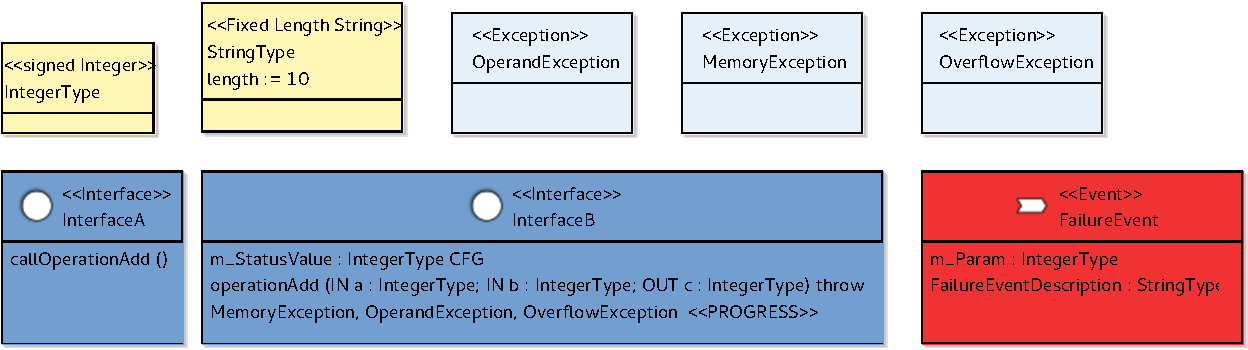
\includegraphics[width=1.0\textwidth]{InterfacesEventsDatasetsDiagram.pdf}
	\caption{Data types, events, exceptions and interfaces diagram}
	\label{fig: Ex. Datatypes etc.}
\end{figure}

\item [Step 3: Definition of component types] Component types namely \texttt{Component\allowbreak\_Caller} and \texttt{Component\allowbreak\_Callee} which form the basis for a reusable software asset are defined as shown in the \cref{fig: Ex. Component types}. 

\texttt{Component\allowbreak\_Caller} has:
\begin{itemize}
\item Provided interface port \texttt{Provided\allowbreak Interface\allowbreak Port} which refers to \texttt{InterfaceA}
\item Required interface port \texttt{Required\allowbreak Interface\allowbreak PortType1} which refers to \texttt{InterfaceB}
\item Required interface port \texttt{Required\allowbreak Interface\allowbreak PortType2} which refers to \texttt{InterfaceB}
\item Event receiver port \texttt{FailureEvent\allowbreak ReceiverPort} which refers to \texttt{Failure\allowbreak Event}
\end{itemize}

The desired interaction kind for the operations in the required interface ports of \texttt{Component\allowbreak\_Caller} are as shown in the \cref{table: NFP RI Ports}

\begin{table}[]
	\centering
	\caption{Desired interaction kind for operations in the required interface ports}
	\label{table: NFP RI Ports}
	\begin{tabular}{|c|c|c|}
		\hline
		\textbf{Required interface ports} & \textbf{Operations} & \textbf{Interaction kind} \\ \hline
		\texttt{RequiredInterfacePortType1} & \begin{tabular}[c]{@{}c@{}}\texttt{OperationAdd}\\ Interface attribute setter\\ Interface attribute getter\end{tabular} & \begin{tabular}[c]{@{}c@{}}\texttt{synchronous}\\ \texttt{synchronous}\\ \texttt{synchronous}\end{tabular} \\ \hline
		\texttt{RequiredInterfacePortType2} & \begin{tabular}[c]{@{}c@{}}\texttt{OperationAdd}\\ Interface attribute setter\\ Interface attribute getter\end{tabular} & \begin{tabular}[c]{@{}c@{}}\texttt{asynchronous}\\ \texttt{asynchronous}\\ \texttt{asynchronous}\end{tabular} \\ \hline
	\end{tabular}
\end{table}

\texttt{Component\allowbreak\_Callee} has:
\begin{itemize}
\item Provided interface port \texttt{Provided\allowbreak Interface\allowbreak Port1} which refers to \texttt{InterfaceB}
\item Provided interface port \texttt{Provided\allowbreak Interface\allowbreak Port2} which refers to \texttt{InterfaceB}
\item Event emitter port \texttt{FailureEvent\allowbreak EmitterPort} which refers to \texttt{FailureEvent}
\end{itemize}

\begin{figure}[h]
	\centering
	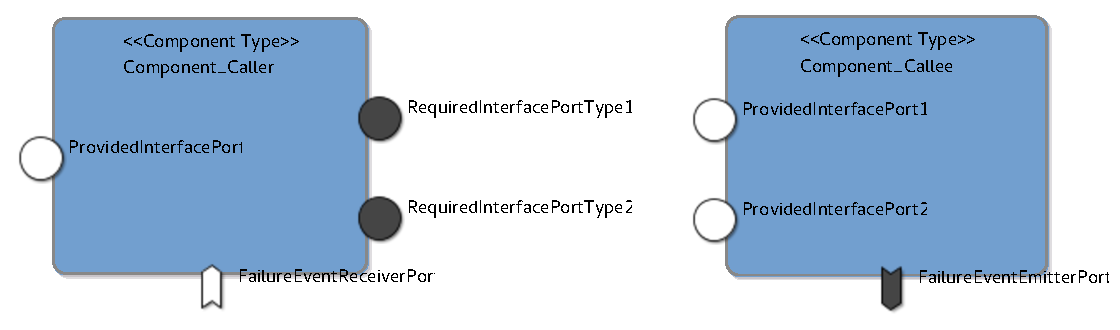
\includegraphics[width=1.0\textwidth]{ComponentTypesDiagram.pdf}
	\caption{Component types diagram}
	\label{fig: Ex. Component types}
\end{figure}

\item [Step 4: Definition of component implementations] Component implementations are created from the component types.

\texttt{Component\allowbreak\_Caller} has one component implementation named as \texttt{Component\allowbreak\_Caller\_impl} and \texttt{Component\allowbreak\_Callee} has one component implementation named as \texttt{Component\allowbreak\_Callee\_impl}. The component implementation \texttt{Component\allowbreak\_Callee\_impl} implements the means to store the attribute \texttt{Param} of \texttt{InterfaceB}, that is exposed through its provided interface ports, namely \texttt{Provided\allowbreak Interface\allowbreak Port1} and \texttt{Provided\allowbreak Interface\allowbreak Port2}.

No maximum memory footprint for component implementations are defined or no detailed design activity of the component implementations are performed as they are not of concern in this Master thesis.

\item [Step 5: Definition of component instances] The component instances are the instances of component implementations \cite{CompBasedProcess}.

Two component instances as shown in \cref{fig: Ex. Component instances} are defined, namely:
\begin{itemize}
\item \texttt{Component\allowbreak\_Caller\_impl\_inst} which is an instantiation of \texttt{Component\allowbreak\_Caller\_impl}
\item \texttt{Component\allowbreak\_Callee\_impl\_inst} which is an instantiation of \texttt{Component\allowbreak\_Callee\_impl}
\end{itemize}

\item [Step 6: Definition of component bindings] Component bindings as shown in \cref{fig: Ex. Component instances} are defined:

\begin{figure}[h]
	\centering
	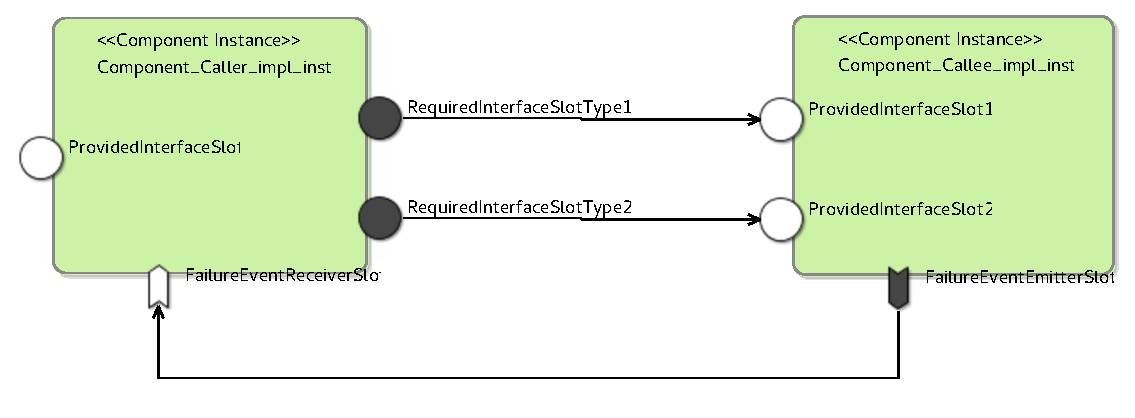
\includegraphics[width=1.0\textwidth]{ComponentInstancesDiagram.pdf}
	\caption{Component instances diagram}
	\label{fig: Ex. Component instances}
\end{figure}

\item [Step 7: Specification of non-functional attributes] The non-functional properties are defined on the component instances and the component bindings defined in the previous step. The non-functional properties language unit of the specification of a metamodel provides a Value Specification Language (VSL) unit, which permits the specification of the the non-functional properties qualified with a measurement unit \cite{SpecMetamodel}. The VSL is used here to define values of non-functional properties with a measurement unit.

For the provided interface slot in the component instance \texttt{Component\allowbreak\_caller\allowbreak\_impl\_inst}, the following non-functional property is specified as shown in \cref{table: NFP PI Ports1}

\begin{table}[]
	\centering
	\caption{Non-functional property for the operation in the provided interface slot}
	\label{table: NFP PI Ports1}
	\begin{tabular}{lll}
		\hline
		\multicolumn{1}{|c|}{\textbf{Provided interface slot}} & \multicolumn{1}{c|}{\textbf{Operation}} & \multicolumn{1}{c|}{\textbf{Non-functional property}} \\ \hline
		\multicolumn{1}{|c|}{\texttt{ProvidedInterfaceSlot}} & \multicolumn{1}{c|}{\texttt{CallOperationAdd}} & \multicolumn{1}{c|}{\texttt{Cyclic}, Period = 2s} \\ \hline
	\end{tabular}
\end{table}

For the provided interface slots in the component instance \texttt{Component\allowbreak\_callee\_impl\_inst}, the following non-functional properties are specified as shown in \cref{table: NFP PI Ports2}

\begin{table}[]
	\centering
	\caption{Non-functional properties for the operations in the provided interface slots}
	\label{table: NFP PI Ports2}
	\begin{tabular}{ccc}
		\hline
		\multicolumn{1}{|c|}{\textbf{Provided interface slots}} & \multicolumn{1}{c|}{\textbf{Operations}} & \multicolumn{1}{c|}{\textbf{Non-functional properties}} \\ \hline
		\multicolumn{1}{|c|}{\texttt{ProvidedInterfaceSlot1}} & \multicolumn{1}{c|}{\begin{tabular}[c]{@{}c@{}}\texttt{OperationAdd}\\ Interface attribute setter\\ Interface attribute getter\end{tabular}} & \multicolumn{1}{c|}{\begin{tabular}[c]{@{}c@{}}\texttt{Protected}\\ \texttt{Protected}\\ \texttt{Unprotected}\end{tabular}} \\ \hline
		\multicolumn{1}{|c|}{\texttt{ProvidedInterfaceSlot2}} & \multicolumn{1}{c|}{\begin{tabular}[c]{@{}c@{}}\texttt{OperationAdd}\\ Interface attribute setter\\ Interface attribute getter\end{tabular}} & \multicolumn{1}{c|}{\begin{tabular}[c]{@{}c@{}}\texttt{Sporadic}, MIAT = 2s\\ \texttt{Protected}\\ \texttt{Protected}\end{tabular}} \\ \hline
		\multicolumn{1}{l}{} & \multicolumn{1}{l}{} & \multicolumn{1}{l}{}
	\end{tabular}
\end{table}

It is important to note that the WCET and deadline values for the operations in the provided interface slots are not handled, as the safeguarding of these properties are not of concern in this Master thesis.

For the event receiver slot in the component instance \texttt{Component\allowbreak\_caller\allowbreak\_impl\allowbreak\_inst}, the following non-functional property is specified as shown in \cref{table: NFP ER Port}

\begin{table}[]
	\centering
	\caption{Non-functional property for event reception}
	\label{table: NFP ER Port}
	\begin{tabular}{ccc}
		\hline
		\multicolumn{1}{|c|}{\textbf{Event receiver slot}} & \multicolumn{1}{c|}{\textbf{\texttt{Event}}} & \multicolumn{1}{c|}{\textbf{Non-functional property}} \\ \hline
		\multicolumn{1}{|c|}{\texttt{FailureEventReceiverSlot}} & \multicolumn{1}{c|}{\texttt{FailureEvent}} & \multicolumn{1}{c|}{\texttt{Protected}} \\ \hline
		\multicolumn{1}{l}{} & \multicolumn{1}{l}{} & \multicolumn{1}{l}{}
	\end{tabular}
\end{table}

\item [Step 8: Definition of the physical architecture] The hardware topology provides a description of the system hardware. As hardware modeling is not of concern in this Master thesis, a simple hardware topology as shown in \cref{fig: Ex. Hardware topology} is considered. 

A processor board with a processor and a processor core is instantiated. Two connection docks are attached to the processor board and a bus is used to connect the connection docks. The component instances are deployed on the processor core and the component bindings are deployed on the bus.

\begin{figure}[h]
	\centering
	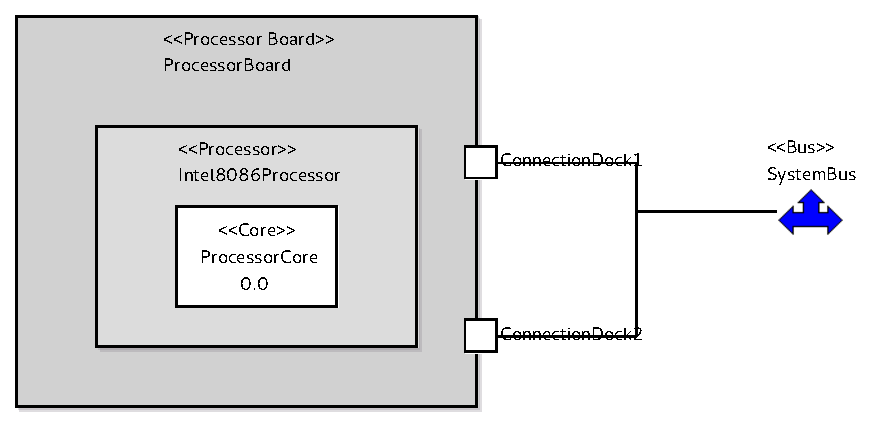
\includegraphics[width=0.8\textwidth]{HardwareDiagram.pdf}
	\caption{Hardware topology diagram}
	\label{fig: Ex. Hardware topology}
\end{figure}
 
\end{description}

This OBSW model is subjected to model validation against the OSRA Specification Compliance and the SCM meta-model compliance, in the OSRA SCM editor \cite{OSRAEditor}. Only after the OBSW model is successfully validated, can the OBSW model be considered as a suitable candidate for automatic generation of infrastructure code \cite{OSRAEditor}.  
   
\subsection{Software design approach for the generated code}
\label{subsection: Software design approach}
This section deals with the software design approach for the generated infrastructure code. Some of the necessary good characteristics of a software such as reusability, separation of concerns and minimal complexity are targeted already at the reference architecture level and it needs to be safeguarded at the generated software level as well. The other main characteristics of the generated software which are of utmost value are \cite{CodeComplete}:
\begin{description}
\item [Testability] The software must be testable and there must be suitable constructs in the generated software which assist in writing automated unit tests or user driven tests to test it. In this Master thesis, it is taken care that the generated C++ classes have corresponding abstract base classes, using which mock classes can be constructed easily for the purpose of testing. More about this is explained in the next chapter which focuses on the results and further scope of this Master thesis
\item [Extensability and Refactorability] The software generated must be loosely coupled so that the entire code base is more resilient to changes and extensions. Dependency injection software design pattern \cite{InvOfCntrlurl} is used wherever appropriate to make the generated software loosely coupled
\item [Portability] The generated software must be portable across systems and environments. The data  types used in the generated software should be portable across multiple platforms and the data type standardizations from C++11 are made use of in the generated software
\item [High fan-in] The generated software is designed in a way that a particular C++ class is used by large number of other C++ classes.
\item [Low-to-medium fan-out] The generated software is designed in a way that a particular C++ class uses not many classes, so that the complexity of the generated software is not too high. Unfortunately, this characteristic is not completely respected in this software design, because the complexity of a particular class depends on the complexity of the user model.      
\end{description}
\ac{uml} class diagrams, wherever appropriate are judiciously used in this section to show a high level representation of the generated C++ classes and datastructures. 

Each of the following sub-sections, is divided into two parts:
\begin{itemize}
\item The first part throws light on the idea of how a mapping of a given model entity to an infrastructural code entity can be done
\item The second part makes the approach clear by taking the reference of our OBSW example model discussed in the previous section  
\end{itemize}

The following sub-sections also include UML class diagrams wherever appropriate. The standard legends from the UML diagrams are used. The following additional legends are introduced:
\begin{itemize}
\item A UML class in dotted notation means that the explanation for that particular has been given in the previous sections or would be given in the following sections 
\item A package notation from UML is used to indicate the namespaces that the respective classes in the UML diagram can be found
\end{itemize}  

\subsubsection{\textbf{Namespaces}}
Namespaces from C++ are used to differentiate component types, component implementations etc. of different components. The names for the namespaces are obtained from the names of the component types in the OBSW model.

\textbf{For our example OBSW model}: Three namespaces, namely \texttt{General}, \texttt{Component\_Caller} and \texttt{Component\_Callee} are created as shown in \cref{fig: PackagesUML}

\begin{figure}[h]
	\centering
	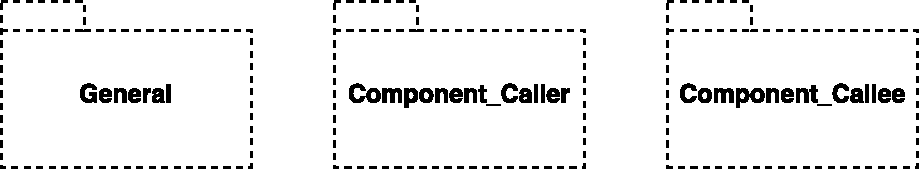
\includegraphics[width=0.5\textwidth]{NamespacesUML.pdf}
	\caption{UML class diagram representation for different namespaces in the example OBSW model}
	\label{fig: PackagesUML}
\end{figure}

\subsubsection{\textbf{Data types and events}}
A data type from the OBSW model is translated into a simple \texttt{typedef} statement from C++.

\textbf{For our example OBSW model}:
\begin{itemize}
\item The data type \texttt{IntegerType}, is translated to \texttt{typedef\allowbreak \ int8\_t IntegerType}
\item The data type \texttt{StringType}, is translated to \texttt{typedef\allowbreak \ std::string StringType} 
\end{itemize}

A subset of all possible data types from the OSRA Component Model can be translated to simple \texttt{typedef} statements as shown above. More information about the subset of data types for which this successfully works is given in the next chapter. 

The exception types from the OBSW models are translated into simple enumeration literals from C++. These exceptions, which can be thrown by a particular operation are grouped under an enumeration. This enumeration is further instantiated in a C++ struct.

\textbf{For our example OBSW model}: The three exceptions \texttt{Operand\allowbreak Exception}, \texttt{Memory\allowbreak Exception} and \texttt{Overflow\allowbreak Exception} are translated to enumeration literals. These exceptions can be thrown by \texttt{OperationAdd}, which is defined in \texttt{InterfaceB}. Hence the enumeration literals, corresponding to the exceptions, are stored together as an enumeration named \texttt{OperationAdd\allowbreak Exception\allowbreak\_InterfaceB} as shown in the \cref{fig: ExceptionsUML}. This exception is further instantiated in a C++ struct \texttt{OperationAdd\allowbreak Report\allowbreak\_InterfaceB} as shown in the \cref{fig: ExceptionsUML} 

\begin{figure}[h]
	\centering
	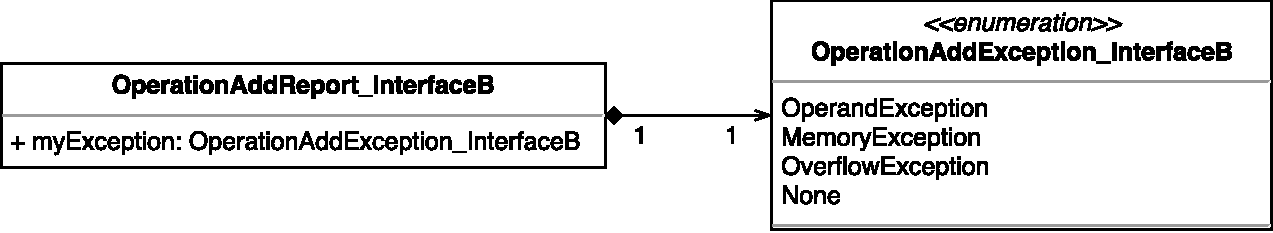
\includegraphics[width=1.0\textwidth]{ExceptionsUML.pdf}
	\caption{UML class diagram representation for exceptions in the example OBSW model}
	\label{fig: ExceptionsUML}
\end{figure}

An event from the OBSW model is mapped to an abstract base class and a corresponding concrete implementation class. As already explained, the abstract base classes hwelp in improving the testability of the generated software. Appropriate setters and getters for the event parameters are declared as pure virtual methods in the abstract base class for the event and they are implemented in their corresponding concrete implementation.

\textbf{For our example OBSW model}: The \texttt{FailureEvent} is mapped as an abstract base class named \texttt{FailureEvent\allowbreak Interface} and concrete implementation class named \texttt{FailureEvent}. Appropriate setters and getters for the event parameters \texttt{Param} and \texttt{Failure\allowbreak Event\allowbreak	Description} are declared as pure virtual methods in the \texttt{FailureEvent\allowbreak Interface} abstract base class and implemented in the \texttt{FailureEvent} concrete implementation class. An UML class diagram representation of the generated classes are as shown in \cref{fig: EventUML}.

\begin{figure}[h]
	\centering
	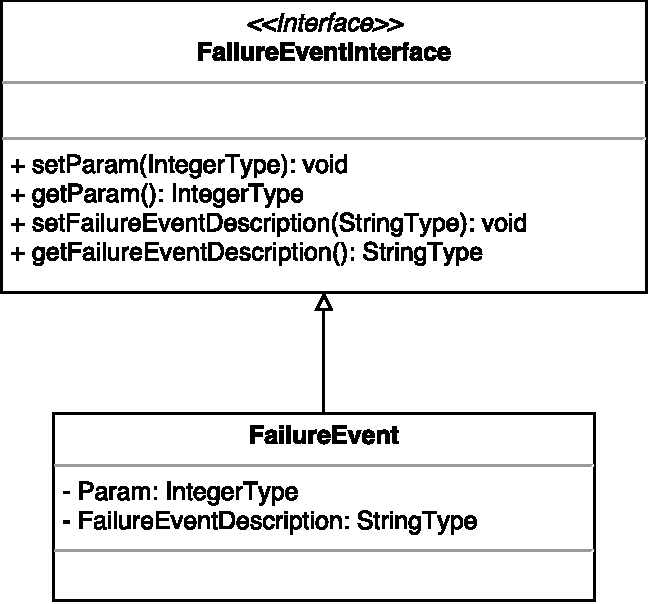
\includegraphics[width=0.6\textwidth]{EventUML.pdf}
	\caption{UML class diagram representation for event in the example OBSW model}
	\label{fig: EventUML}
\end{figure}    

All the infrastructure code entities mentioned above are present in the namespace \texttt{General}.  

\subsubsection{\textbf{Interfaces}}
An interface can be mapped to a C++ abstract base class, as in \cite{EvoRAVCodeAr}. Constituents of this abstract base class are:

\begin{itemize}
\item For each interface operation, a pure virtual method is declared in the interface class. The names and data types of the input parameters for this pure virtual method corresponds to the names and data types of the interface operation parameters. The operation parameters, with \texttt{ParameterDirectionKind} as \texttt{in} are translated to constant references and the operation parameters with \texttt{ParameterDirectionKind} as \texttt{out} or \texttt{inout} are translated to plain references. 
\item For each interface attribute parameter of type \texttt{CFG}:
\begin{itemize}
\item A class variable of name and data type corresponding to the name and data type of interface attribute is added
\item Pure virtual setter and getter methods for the interface attribute are declared. The data types and names of the input parameters in the setter and getter methods mimic the name and data type of the interface attribute.
\end{itemize} 
\item For each interface attribute parameter of type \texttt{MIS}, which is fixed and is not variable \cite{SpecMetamodel}: 
\begin{itemize}
\item A \texttt{const} class variable of name and data type corresponding to the name and data type of interface attribute is added
\item No getter and setter methods are added
\end{itemize}
\item For each interface attribute of type \texttt{DAT}, which are modifiable by the component only and not by external entities \cite{SpecMetamodel}:
\begin{itemize}
\item A class variable of name and data type corresponding to the name and data type of interface attribute is added
\item No getter and setter methods are added  
\end{itemize}   
\end{itemize}

\textbf{For our example OBSW model} The C++ classes shown in \cref{fig: InterfacesUML} are generated:
\begin{itemize}
\item \texttt{InterfaceA} along with the operation \texttt{CallOperationAdd} is mapped to an abstract base class \texttt{InterfaceA} with a pure virtual method \texttt{CallOperationAdd}. 
\item \texttt{InterfaceB} has one operation \texttt{OperationAdd} and one interface attribute parameter \texttt{StatusValue} of type \texttt{CFG}. These are mapped to an abstract base class named \texttt{InterfaceB} with the following pure virtual methods:
\begin{itemize}
\item \texttt{OperationAdd} with two input parameters of type \texttt{const\allowbreak \ IntegerType\&} and one input parameter of type \texttt{IntegerType\&}
\item getter method for the interface attribute \texttt{StatusValue} with an input parameter of type \texttt{IntegerType\&}
\item setter method for the interface attribute \texttt{StatusValue} with an input parameter of type \texttt{const\allowbreak \ IntegerType\&}
\end{itemize} 
\end{itemize}

\begin{figure}[h]
	\centering
	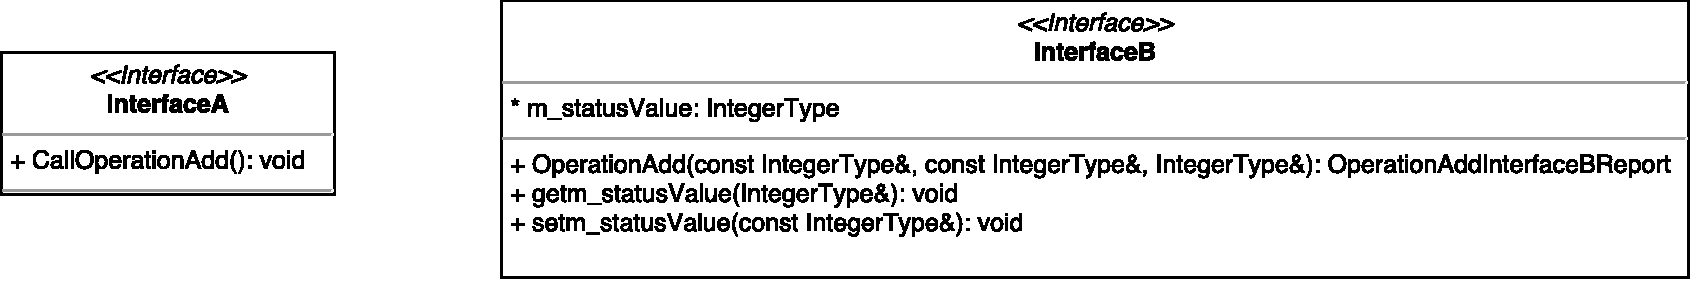
\includegraphics[width=1.0\textwidth]{InterfacesUML.pdf}
	\caption{UML class diagram representation for interfaces in the example OBSW model}
	\label{fig: InterfacesUML}
\end{figure}

Because of the corner case that multiple interfaces can have exactly same operations, it is necessary to refine these interfaces using the interface helper abstract base classes as shown in \cref{fig: Interface helpers UML}. In each interface helper class:
\begin{itemize}
\item Implementations for all the inherited pure virtual methods from the parent interface are provided
\item The implementations consist of simple method calls to new pure virtual methods
\item These new pure virtual methods have method signatures same as the pure virtual methods that are inherited and implemented. However, it is important to note that the names of these new pure virtual methods are different from the inherited pure virtual methods, as shown in the \cref{Listing: Interface helper Impl} 
\end{itemize}

\begin{figure}[h]
	\centering
	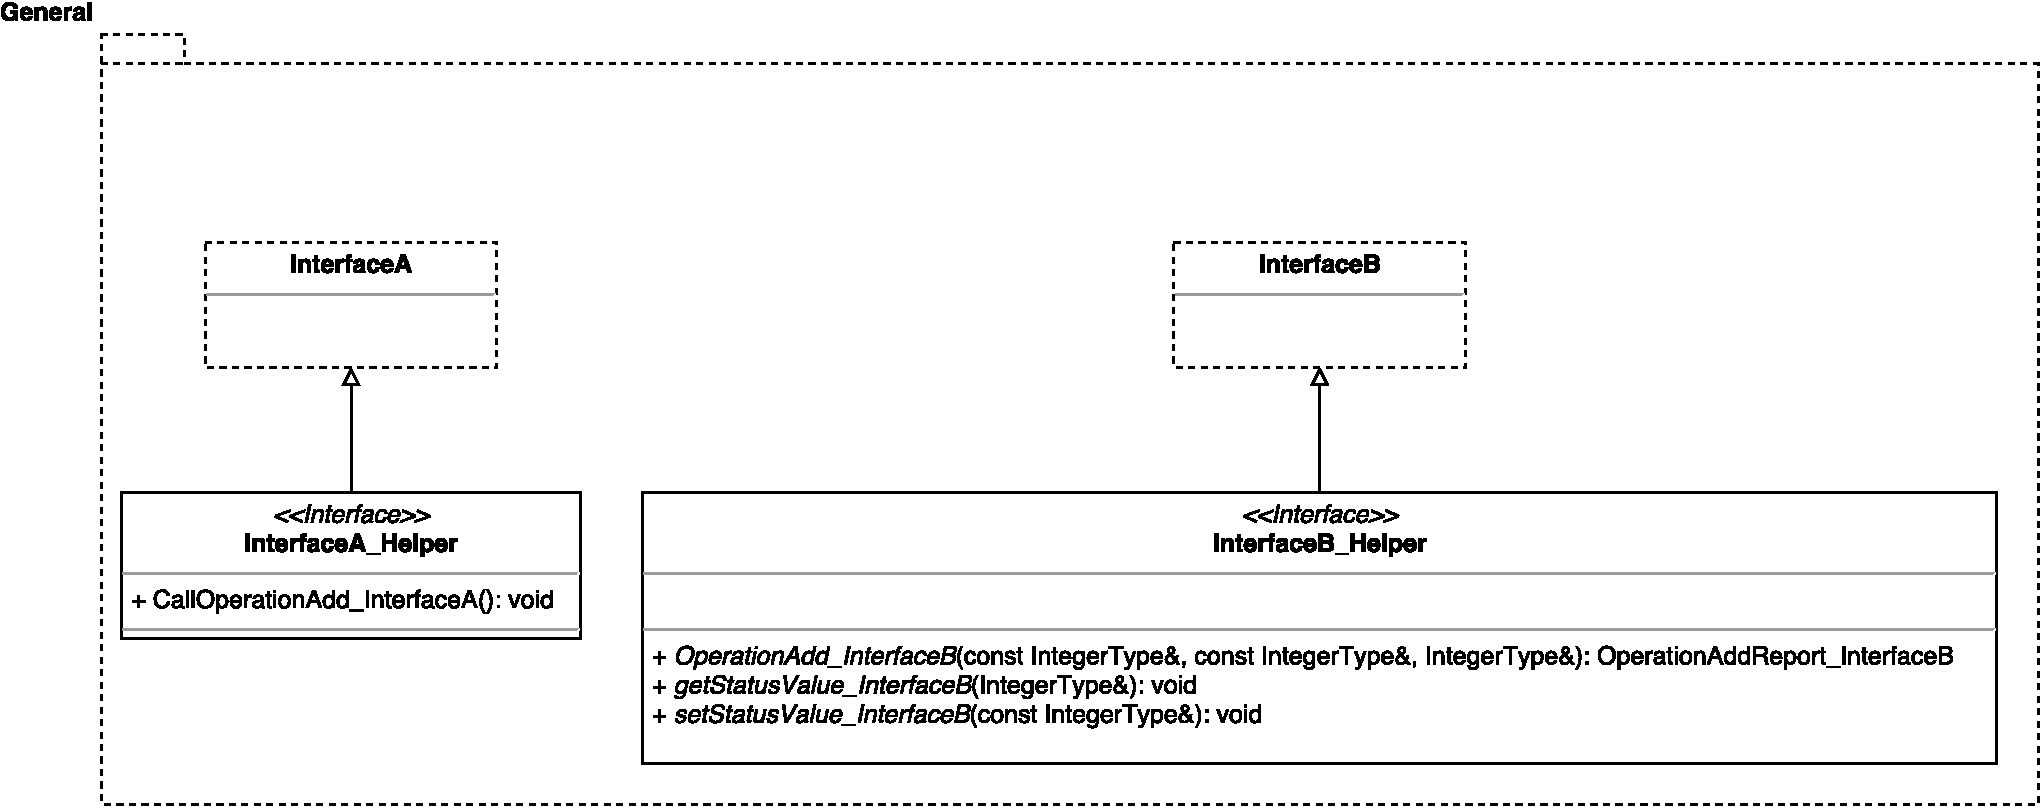
\includegraphics[width=0.8\textwidth]{InterfaceHelpersUML.pdf}
	\caption{UML class diagram representation for interface helpers in the example OBSW model}
	\label{fig: Interface helpers UML}
\end{figure}

\begin{Listing}
\begin{lstlisting}[language=C++]
class InterfaceA {
public:
	InterfaceA(){}
	virtual ~InterfaceA(){}
	virtual void callOperationAdd(void) = 0;
};

class InterfaceA_Helper: public InterfaceA {
public:
	InterfaceA_Helper(){}
	virtual ~InterfaceA_Helper(){}
	virtual void callOperationAdd_InterfaceA(void) = 0; //New pure virtual method
	virtual void callOperationAdd(void)final {return (callOperationAdd_InterfaceA());}
};
\end{lstlisting}
\caption{Code excerpt from the generated code for \texttt{InterfaceA\allowbreak\_Helper}}
\label{Listing: Interface helper Impl}
\end{Listing}

\textbf{For our example OBSW model}:
\begin{itemize}
\item \texttt{InterfaceA\allowbreak\_Helper} is defined, which inherits from the interface \texttt{InterfaceA} and which implements the pure virtual method in the parent interface \texttt{InterfaceA}. The implementation contains a simple call to a new pure virtual method added to the original method name from the parent interface as shown in the \cref{Listing: Interface helper Impl}.

\item \texttt{InterfaceB\allowbreak\_Helper} is defined, which inherits from the interface \texttt{InterfaceB} and which implements all the pure virtual methods in the parent interface \texttt{InterfaceB}. Each implementation contain a simple call to the new pure virtual methods added. The \texttt{InterfaceB\allowbreak\_Helper} class is designed and implemented the same way as \texttt{InterfaceA\allowbreak\_Helper} is designed in the code excerpt in \cref{Listing: Interface helper Impl}   
\end{itemize}

The combined effect is that now, more than one original parent interfaces (resembling model entities) can have same operations and interface attributes. The refined interfaces redefine the methods from the original parent interfaces, so that there are no confusions between operations from different interfaces. Of course, a straight forward solution would have been to incorporate the concept of namespaces from C++, but it is not suitable for this design and the reason is explained later in this section. 

For each interface operation and interface attribute in an interface, a C++ struct is defined to carry around the values of the operation parameters or the values of the interface attributes. These data structures come in handy, when the interface operations or interface attribute access operations need to be accessed asynchronously. The data structures also hold general purpose polymorphic function wrappers from C++11 standard to store the call-back functions wherever appropriate. 

\textbf{For our example OBSW model}:
\begin{itemize}
\item A struct \texttt{OperationAdd\allowbreak Struct\_\allowbreak InterfaceB} is defined as shown in \cref{fig: Operation structs UML}
\item A struct \texttt{StatusValue\allowbreak Struct\_\allowbreak InterfaceB} is defined as shown in \cref{fig: Operation structs UML}
\end{itemize} 

\begin{figure}[h]
	\centering
	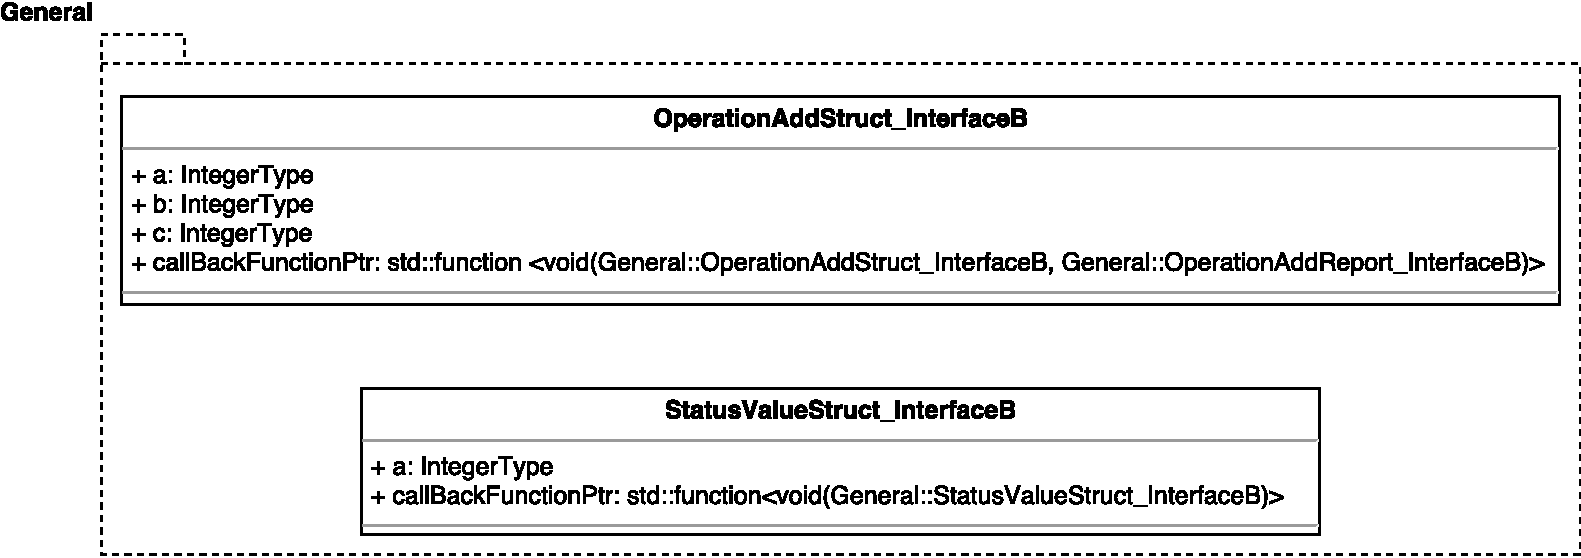
\includegraphics[width=0.8\textwidth]{OperationStructsUML.pdf}
	\caption{UML class diagram representation of data structures for interface operation and interface attribute in the example OBSW model}
	\label{fig: Operation structs UML}
\end{figure} 

All the infrastructure code entities mentioned above are present in the namespace \texttt{General}.

\subsubsection{\textbf{Parameter channels and parameter queues}}
The data structures which are defined to carry around the values of the operation parameters or values of the interface attributes, need to be pushed onto parameter channels, each one of which is supported in the back end by corresponding parameter queue.

\textbf{For our example OBSW model}: \texttt{Parameter\allowbreak Channel} and \texttt{Parameter\allowbreak Queue} C++ classes as shown in \cref{fig: Parameter channel UML} are defined. These classes can be reused for any OBSW model. 

\begin{figure}[h]
	\centering
	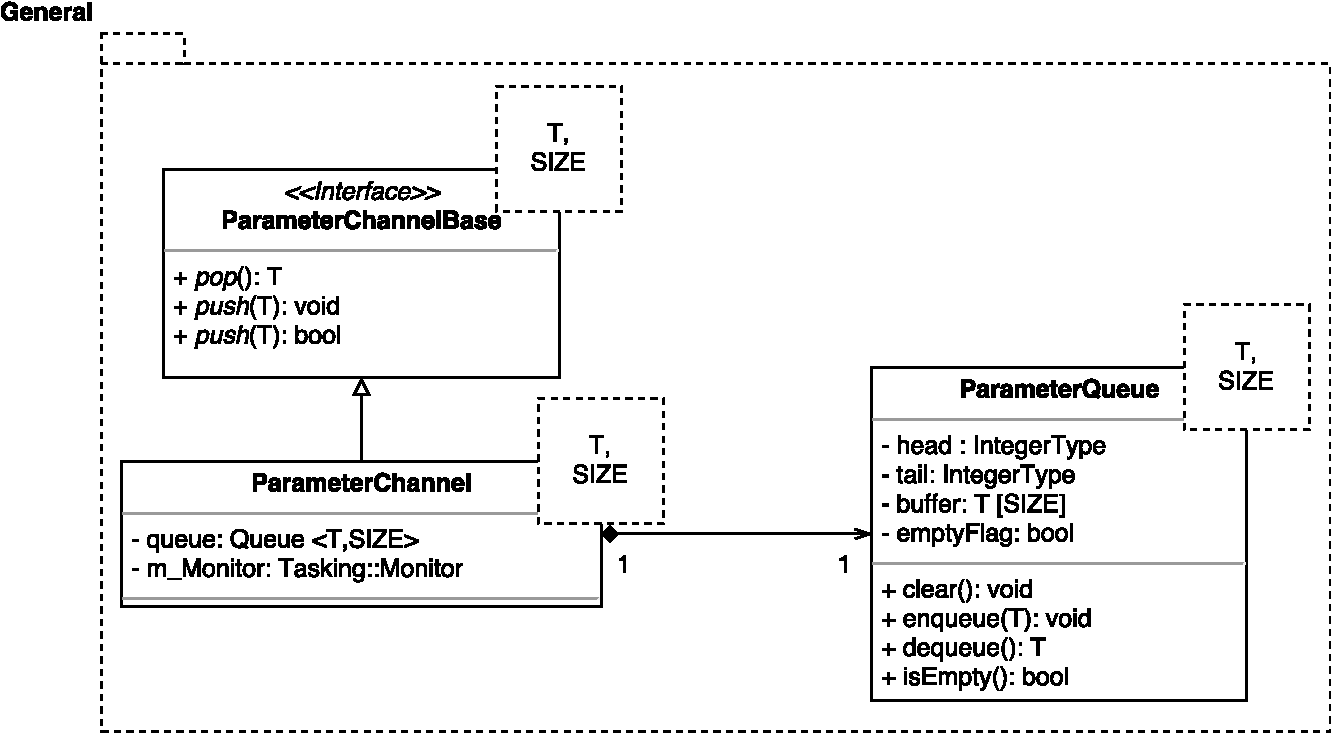
\includegraphics[width=1.0\textwidth]{ParameterChannelQueue.pdf}
	\caption{UML class diagram representation of parameter channel and parameter queue in the example OBSW model}
	\label{fig: Parameter channel UML}
\end{figure}

All the infrastructure code entities mentioned above are present in the namespace \texttt{General}.   

\subsubsection{\textbf{Event emitter ports and event receiver ports}}
The event emitter port for a particular event is mapped as an abstract base class and a corresponding concrete implementation class in C++. The event receiver port for a particular event is mapped only as an abstract base class. The abstract base class for event receiver port also contains pure virtual methods in order to safely interleave the reception of events.  

\textbf{For our example OBSW model}: The \texttt{FailureEvent\allowbreak EmitterPort} is mapped as a pair of abstract base class and a concrete implementation class as shown in \cref{fig: Event emitter port UML}.  

\textbf{For our example OBSW model}: The \texttt{FailureEvent\allowbreak ReceiverPort} is mapped to an abstract base class as shown in \cref{fig: Event receiver port UML}.

\begin{figure}[h]
	\centering
	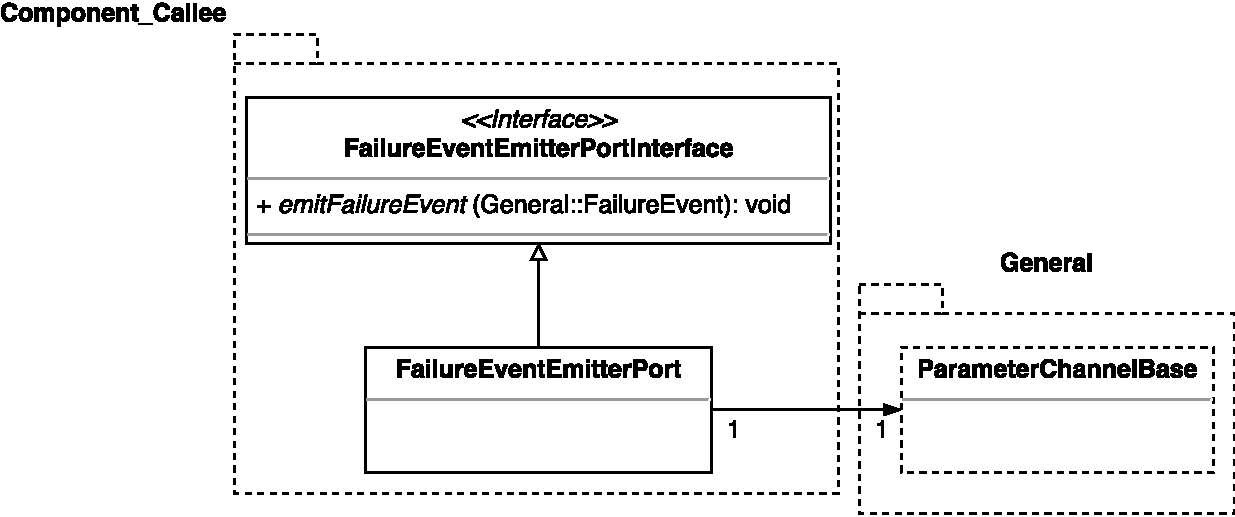
\includegraphics[width=1.0\textwidth]{EventEmitterPortUML.pdf}
	\caption{UML class diagram representation of event emitter port in the example OBSW model}
	\label{fig: Event emitter port UML}
\end{figure}

\begin{figure}[h]
	\centering
	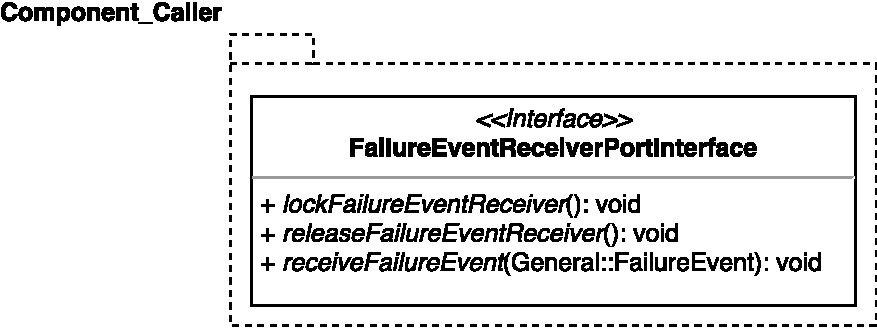
\includegraphics[width=0.8\textwidth]{EventReceiverPortUML.pdf}
	\caption{UML class diagram representation of event receiver port in the example OBSW model}
	\label{fig: Event receiver port UML}
\end{figure} 

The \texttt{FailureEvent\allowbreak Emitter\allowbreak Port\allowbreak Interface} and \texttt{FailureEvent\allowbreak Emitter\allowbreak Port} classes are defined in the namespace \texttt{Component\allowbreak \_Callee}. 

The \texttt{FailureEvent\allowbreak Receiver\allowbreak Port\allowbreak Interface} is defined in the namespace \texttt{Component\allowbreak\_Caller}.

\subsubsection{\textbf{Component types}}
A component type can be mapped to an abstract base class in C++. A component type must provide all the operations that are listed in the provided interfaces of the component \cite{CompBasedProcess}. Hence it inherits from all the interface helper classes which are referenced by its provided interfaces as in \cite{EvoRAVCodeAr} 

This is where interface helper classes, with redefined operations come in handy, because C++ does not distinguish between operations with same signatures, although they are inherited from different namespaces. A component type must also inherit from the mapped abstract base classes for event receiver ports.

A component type must also have pure virtual methods which obtain and release the semaphores for the concurrent access of different operations that it provides. In addition to these, pure virtual methods need to be added, which act as call-back functions for the operations, that the component type's required interface ports request to be released asynchronously.   

\textbf{For our example OBSW model}:
\begin{itemize}
\item As shown in \cref{fig: Component type Caller UML} \texttt{ComponentType} in the namespace \texttt{Component\_Caller} inherits from the \texttt{InterfaceA\allowbreak\_Helper} and also inherits from the abstract base class \texttt{FailureEvent\allowbreak ReceiverPort\allowbreak Interface}. 
It has pure virtual methods meant for:

\begin{itemize}
\item Obtaining and releasing of semaphores for concurrent accesses of the operation \texttt{CallOperationAdd\allowbreak\_InterfaceA}
\item Call-back function for the operation \texttt{OperationAdd}
\item Call-back function for the getter operation of the interface attribute \texttt{StatusValue} 
\end{itemize}

\item A shown in \cref{fig: Component type Callee UML} \texttt{ComponentType} in the namespace \texttt{Component\_Callee} inherits from the \texttt{InterfaceB\allowbreak\_Helper}. 
It has pure virtual methods meant for:

\begin{itemize}
\item Obtaining and releasing of semaphores for concurrent access of the operation {OperationAdd\allowbreak\_InterfaceB}
\item Obtaining and releasing of semaphores for concurrent access of the setter and getter operations for the interface attribute \texttt{StatusValue}
\end{itemize}   
\end{itemize}

\begin{figure}[h]
	\centering
	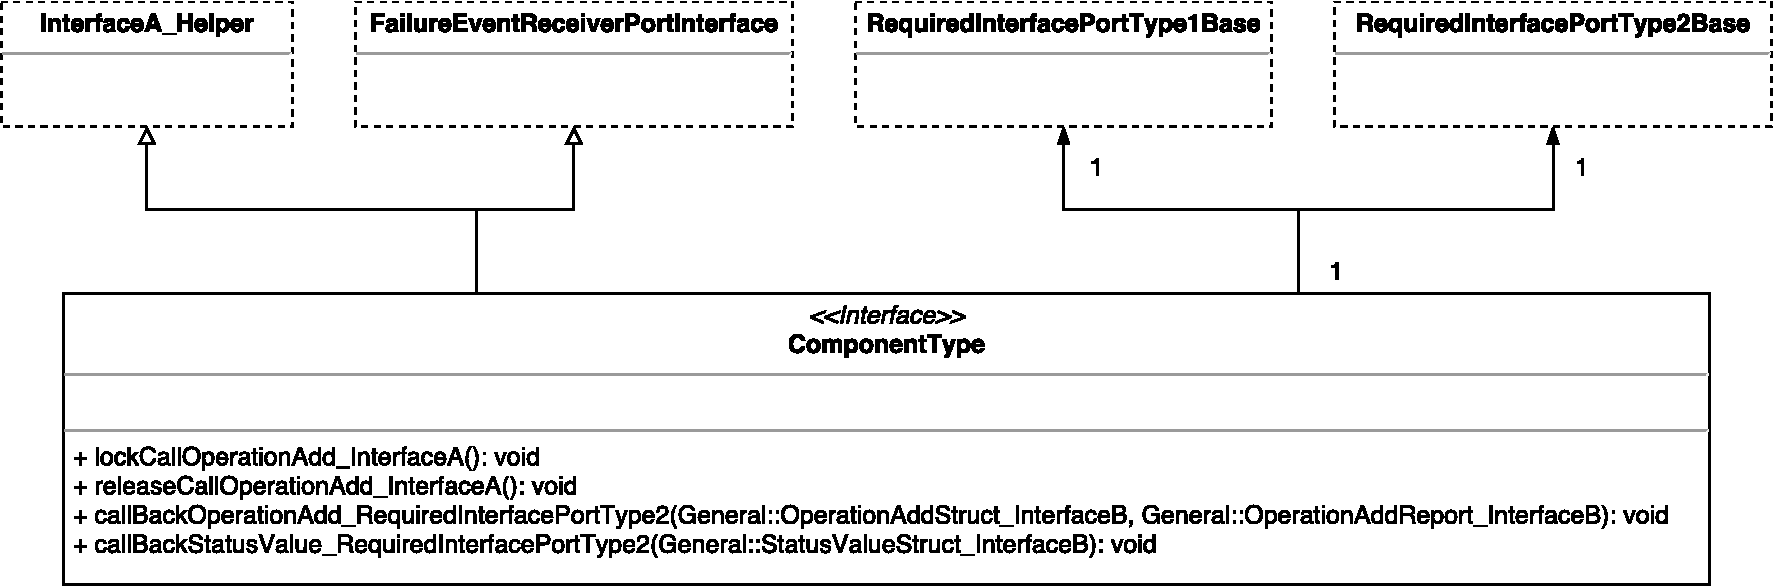
\includegraphics[width=1.0\textwidth]{ComponentTypeCallerUML.pdf}
	\caption{UML class diagram representation of component type for \texttt{Component\allowbreak\_Caller} in the example OBSW model}
	\label{fig: Component type Caller UML}
\end{figure} 

\begin{figure}[h]
	\centering
	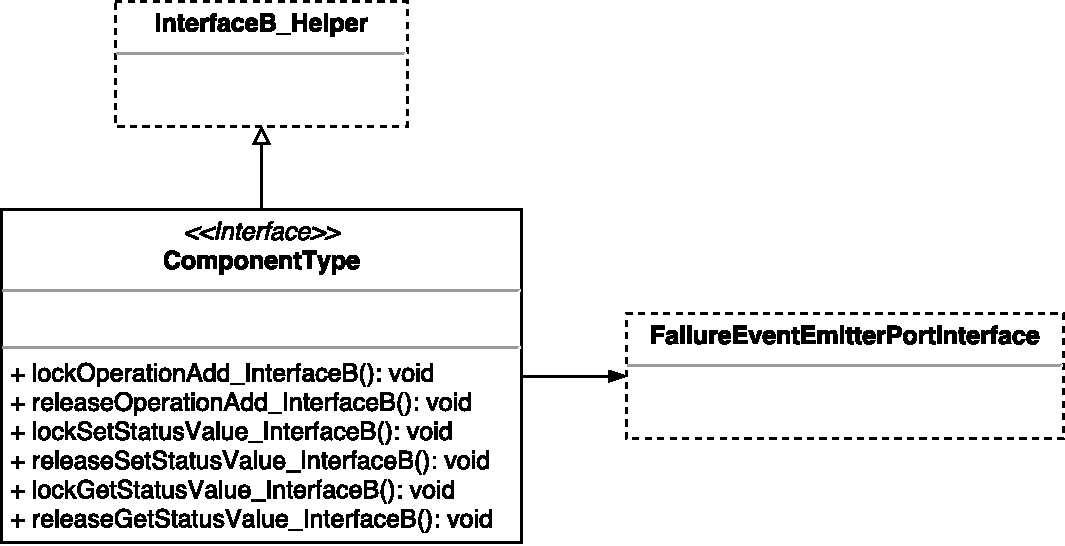
\includegraphics[width=0.8\textwidth]{ComponentTypeCalleeUML.pdf}
	\caption{UML class diagram representation of component type for \texttt{Component\allowbreak\_Callee} in the example OBSW model}
	\label{fig: Component type Callee UML}
\end{figure} 

\subsubsection{\textbf{Required interface ports}}
A required interface port is mapped as an abstract base class and a corresponding concrete implementation class in C++. The required interface subsumed by a particular component type has various operations that it might request and each operation has information specified whether the required interaction kind is \texttt{synchronous} or \texttt{asynchronous} \cite{SpecMetamodel}\cite{CompBasedProcess}. 

Each required interface port refers to one interface type and for each operation in the required interface port, a pure virtual method is added to the abstract base class. The signatures of these methods depend on whether the operations would be requested with an asynchronous release pattern or synchronous release pattern.

In case of interface operations:
\begin{itemize}
\item If the desired interaction kind for the operation is \texttt{synchronous}, then the signature of the method in the abstract base class is same as the corresponding method in the abstract base class for the interface, as shown in \cref{fig: Required interface port1 UML}.
\item If the desired interaction kind for the operation is \texttt{asynchronous}, then the signature of the method in the abstract base class bears no resemblance to the corresponding method in the abstract base class for the interface. It is changed as shown in \cref{fig: Required interface port2 UML} to replace the \texttt{out} and \texttt{inout} parameters with a single pointer to the desired call-back function 
\end{itemize}

In case of interface attributes:
\begin{itemize}
\item For the setter operation, signature of the method in the abstract class is same as the corresponding method in the abstract base class for the interface, as shown in \cref{fig: Required interface port1 UML} and \cref{fig: Required interface port2 UML}
\item If the desired interaction kind for the getter operation is \texttt{synchronous}, then the signature of the method in the abstract class is same as the corresponding method in the abstract base class for the interface, as shown in \cref{fig: Required interface port1 UML}. 
\item If the desired interaction kind for the getter operation is \texttt{asynchronous}, then the signature of the method in the abstract base class bears no resemblance to the corresponding method in the abstract base class for the interface. It is changed as shown in \cref{fig: Required interface port2 UML} to replace the method parameter with a single pointer to the desired call-back function  
\end{itemize} 

The concrete implementation of any method, for example, as the one shown in the code excerpt in \cref{Listing: Required interface port1 Impl} is fairly simple, if the desired interaction kind for the corresponding operation is \texttt{synchronous}. The implementation consists of a simple method call to the corresponding operation in the abstract base class of the bound provided interface port.

\begin{Listing}
\begin{lstlisting}[language=C++]
General::OperationAddReport_InterfaceB RequiredInterfacePortType1::OperationAdd (const IntegerType& a,const IntegerType& b,IntegerType& c) {
	General::OperationAddReport_InterfaceB myReport;
	myReport = m_targetProvidedInterfacePort.OperationAdd(a,b,c); //Simple method call
	return myReport;
}
\end{lstlisting}
\caption{Code excerpt from the generated code for requesting service \texttt{OperationAdd} in \texttt{Required\allowbreak InterfacePort\allowbreak Type1}}
\label{Listing: Required interface port1 Impl}
\end{Listing}

The concrete implementation for any method, for example, the one as shown in code excerpt in \cref{Listing: Required interface port2 Impl} is fairly complex, if the desired interaction kind for the corresponding operation is \texttt{asynchronous}. It would do the following things: 
\begin{itemize}
\item Make local copies of all the method parameters (if any)
\item Pack them in the instances of data structures designed to carry the corresponding parameters
\item Simple method call to the corresponding operation in the abstract base class of the bound provided interface port
\end{itemize}

\begin{Listing}
\begin{lstlisting}[language=C++]
void RequiredInterfacePortType2::getStatusValue(callBackStatusValue_RequiredInterfacePortType2 callBackFunctionPtr) {
	StatusValueStruct_InterfaceB myStruct; 
	myStruct.callBackFunctionPtr = std::bind(callBackFunctionPtr,m_myCallerInstance,std::placeholder::_1);
	m_targetProvidedInterfaceSlot.getStatusValue_Receiver(myStruct); //Simple method call
}
\end{lstlisting}
\caption{Code excerpt from the generated code for interface attribute \texttt{StatusValue} access in \texttt{Required\allowbreak InterfacePort\allowbreak Type2}}
\label{Listing: Required interface port2 Impl}
\end{Listing}

It is clear that local copies of the method parameters need to be made because the desired interaction kind is \texttt{asynchronous}.             

\textbf{For our example OBSW model}: The following C++ classes are defined:
\begin{itemize}
\item \texttt{RequiredInterface\allowbreak PortType1Base} abstract base class and its corresponding \texttt{Required\allowbreak InterfacePort\allowbreak Type1} concrete implementation class.
\item \texttt{RequiredInterface\allowbreak PortType2Base} abstract base class and its corresponding \texttt{Required\allowbreak InterfacePort\allowbreak Type2} concrete implementation class
\end{itemize}

The \texttt{RequiredInterface\allowbreak PortType1Base} and \texttt{RequiredInterface\allowbreak PortType2Base} have pure virtual methods as per the general description and they have to be implemented in the concrete implementation classes \texttt{Required\allowbreak InterfacePort\allowbreak Type1} and \texttt{Required\allowbreak InterfacePort\allowbreak Type2} respectively. The concrete implementations are in line with the description as in the general case above.

\begin{figure}[h]
	\centering
	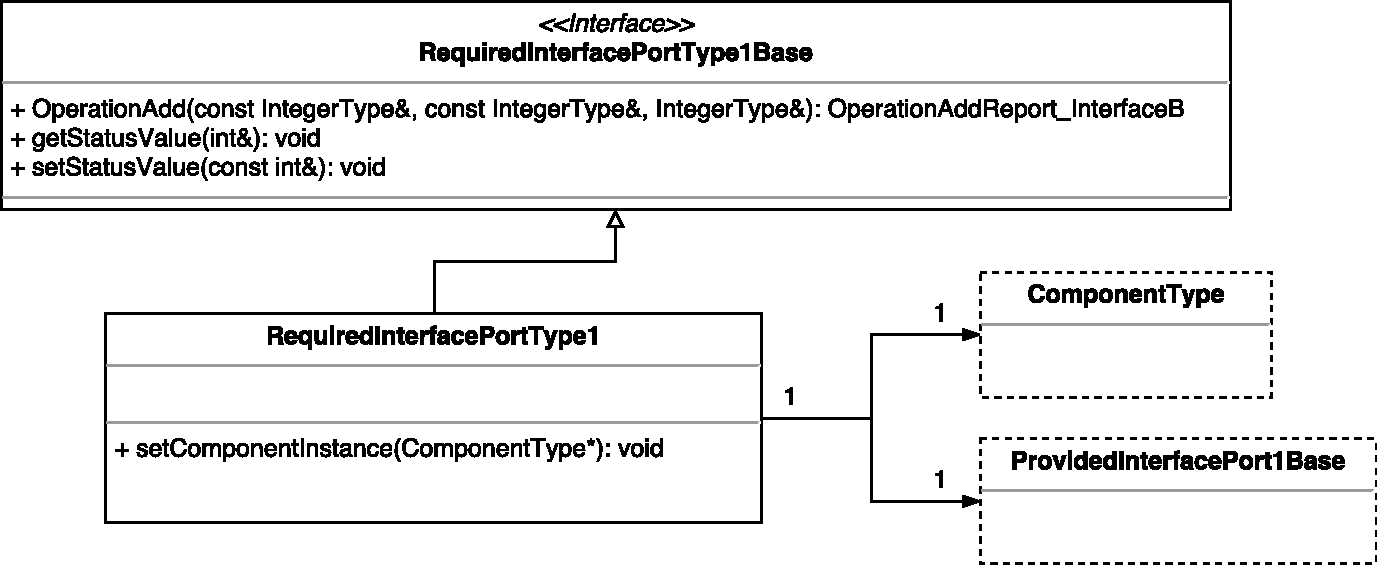
\includegraphics[width=1.0\textwidth]{RequiredInterfacePort1UML.pdf}
	\caption{UML class diagram representation of \texttt{Required\allowbreak InterfacePort\allowbreak Type1} for \texttt{Component\allowbreak\_Caller} in the example OBSW model}
	\label{fig: Required interface port1 UML}
\end{figure}

\begin{figure}[h]
	\centering
	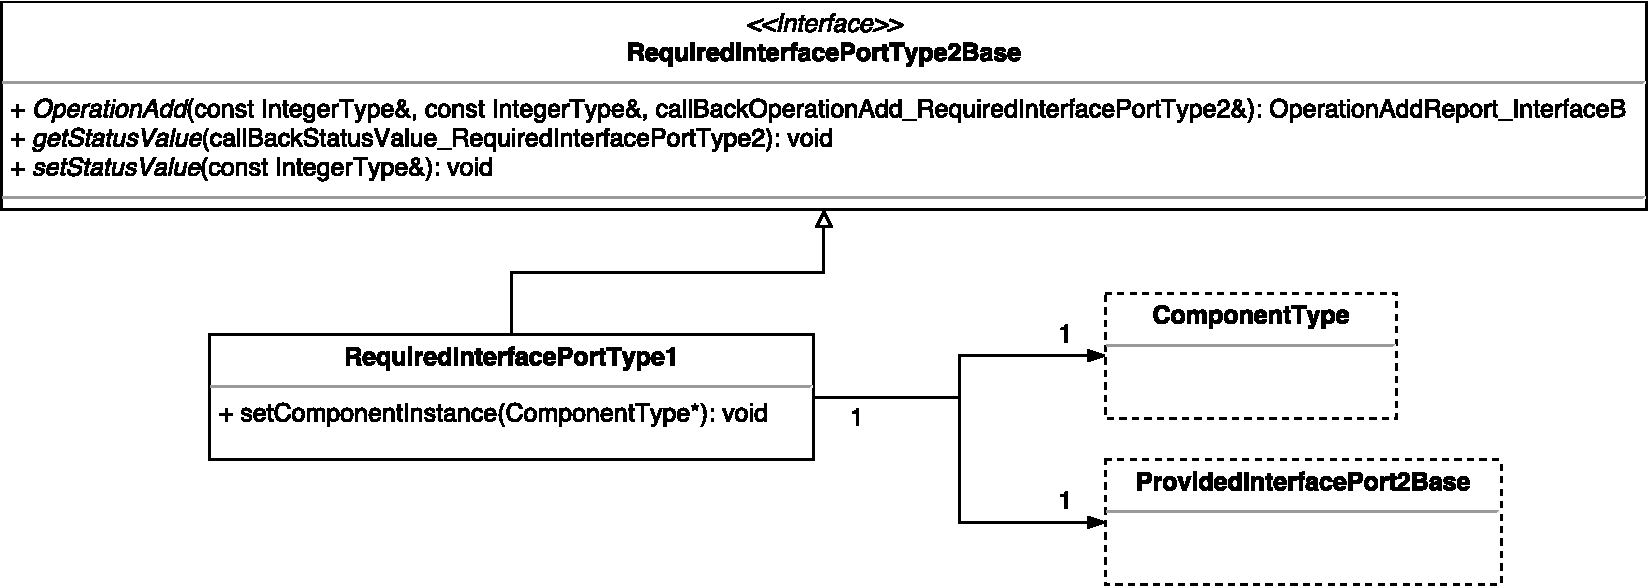
\includegraphics[width=1.0\textwidth]{RequiredInterfacePort2UML.pdf}
	\caption{UML class diagram representation of \texttt{Required\allowbreak InterfacePort\allowbreak Type2} for \texttt{Component\allowbreak\_Caller} in the example OBSW model}
	\label{fig: Required interface port2 UML}
\end{figure}

All the C++ classes mentioned above are present in the namespace \texttt{Component\allowbreak\_Caller}. As the component type \texttt{Component\allowbreak\_Callee} does not have any required interface ports, no C++ classes related to required interface ports are defined in the namespace \texttt{Component\allowbreak\_Callee}. 

\subsubsection{\textbf{Component implementations}}
A component implementation can be mapped in C++ as a concrete implementation of its abstract component type base class. as in \cite{EvoRAVCodeAr}. It implements all the pure virtual methods that are inherited from its component type. It also has actual instances of semaphores for allowing safe concurrent accesses to the implemented methods and for safe interleaving between concurrent receptions of events of the same type.

In case of components that promote multiple provided interface ports which refer to the same interface type, it is necessary to provide multiple implementations for the operations in the provided interfaces. In order to solve this problem a class hierarchy as shown in \cref{fig: Component implementation Callee UML} is decided upon in this Master thesis:

\begin{itemize}
\item A component implementation abstract base class is designed which contains implementations for inherited pure virtual methods related to acquiring and releasing of semaphores. Also the inherited pure virtual methods which are provided only once are implemented here
\item The Component implementation abstract base class is further extended by dummy abstract base classes. A dummy base class is added for each of the provided interface ports which refer to the same interface type. These dummy abstract base classes help in testing of the implementations of the services which are provided more than once by multiple provided interfaces. With the help of these dummy abstract base classes, mock implementation classes can be easily created and used for testing \cite{InvOfCntrlurl}  
\item These dummy abstract base classes are extended by concrete implementation classes which provide different concrete implementations for all the inherited operations except the ones, which are already implemented in the component implementation abstract base class
\item As it is a necessity to have only one instantiable concrete implementation per component \cite{EvoRAVCodeAr}\cite{SpecMetamodel}\cite{CompBasedProcess}, all the concrete implementations are inherited one last time in a component implementation class. This instance is now deployable on the hardware platform
\end{itemize}
 
\textbf{For our example OBSW model}:
\begin{itemize}
\item \texttt{Component\allowbreak Implementation} concrete implementation class in the namespace \texttt{Component\_Caller} inherits from the abstract base class \texttt{Component\_Type} in namespace \texttt{Component\allowbreak\_Caller} as shown in \cref{fig: Component implementation Caller UML}. It provides implementation for all the inherited pure virtual methods
\item Because the \texttt{ComponentType} in the namespace \texttt{Component\_Callee} has two provided interface ports namely, \texttt{Provided\allowbreak Interface\allowbreak Port1} and \texttt{Provided\allowbreak Interface\allowbreak Port2}, which refer to \texttt{InterfaceB}, the following classes as shown in \cref{fig: Component implementation Callee UML} are created in the namespace \texttt{Component\_Callee}:
\begin{itemize}
\item \texttt{ComponentImplementation\allowbreak Base} which is an abstract base class, but provides implementation for inherited pure virtual methods related to acquiring and releasing of semaphores
\item \texttt{Component\allowbreak Implementation\allowbreak Base\_\allowbreak Provided\allowbreak Interface\allowbreak Port1\allowbreak} and \texttt{Component\allowbreak Implementation\allowbreak Base\_\allowbreak Provided\allowbreak Interface\allowbreak Port2\allowbreak} which are two dummy abstract base classes
\item \texttt{Component\allowbreak Implementation\_\allowbreak Provided\allowbreak Interface\allowbreak Port1} and \texttt{Component\allowbreak Impl\allowbreak emen\allowbreak tation\_\allowbreak Provided\allowbreak Interface\allowbreak Port2} which provide different implementations for all the inherited operations except the ones implemented in \texttt{Component\allowbreak Implementation\allowbreak Base}
\item \texttt{Component\allowbreak Implementation} which inherits from both \texttt{Component\allowbreak Implemen\allowbreak tation\allowbreak Provided\allowbreak Interface1} and \texttt{Component\allowbreak Implementation\allowbreak Provided\allowbreak Inter\allowbreak face2}
\end{itemize}   
\end{itemize}

\begin{figure}[h]
	\centering
	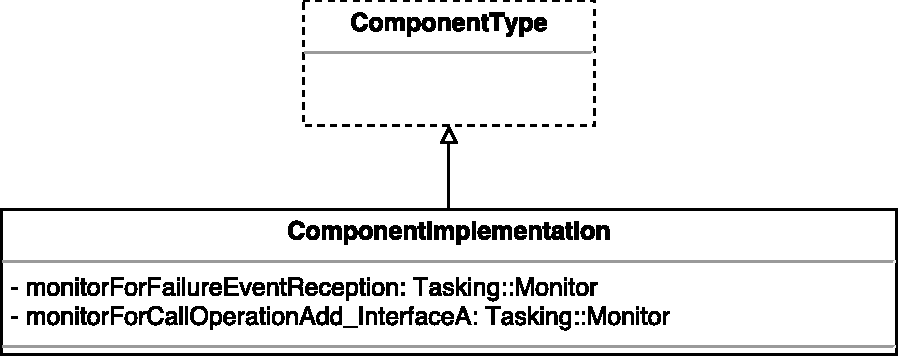
\includegraphics[width=0.8\textwidth]{ComponentImplementationCallerUML.pdf}
	\caption{UML class diagram representation of component implementation for \texttt{Component\_\allowbreak Caller} in the example OBSW model}
	\label{fig: Component implementation Caller UML}
\end{figure} 

\begin{figure}[h]
	\centering
	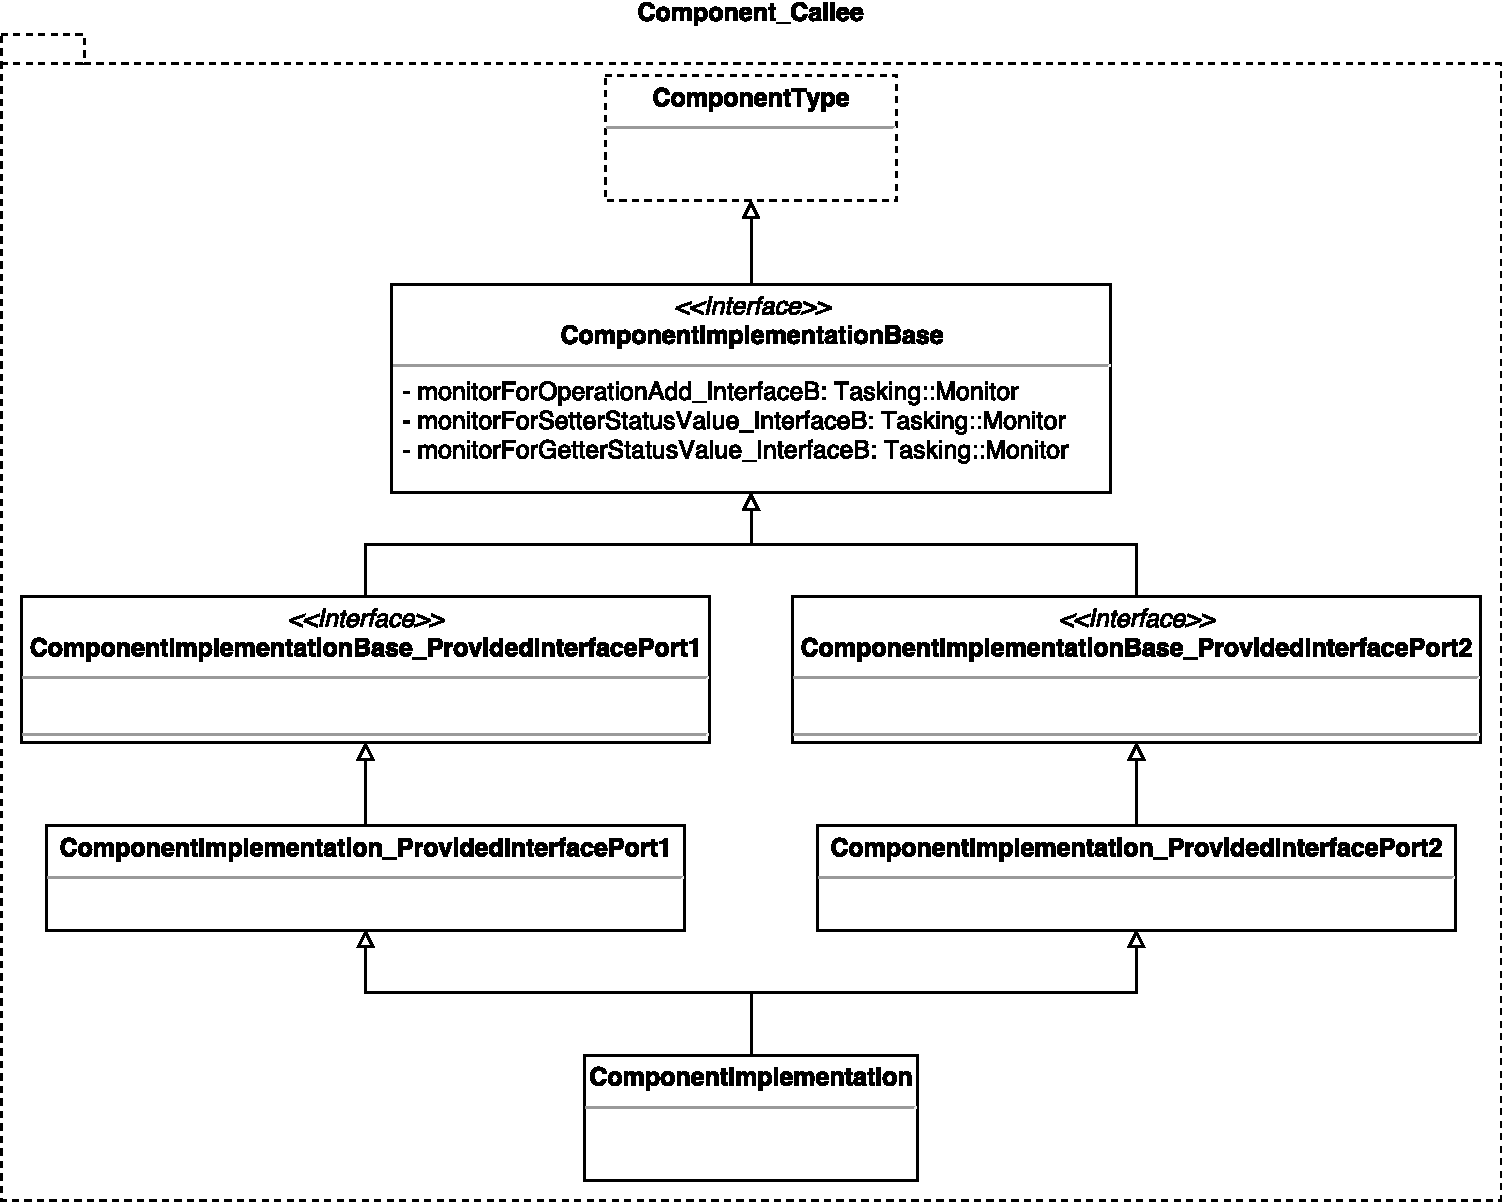
\includegraphics[width=1.0\textwidth]{ComponentImplementationCalleeUML.pdf}
	\caption{UML class diagram representation of component implementations for \texttt{Component\_\allowbreak Callee} in the example OBSW model}
	\label{fig: Component implementation Callee UML}
\end{figure}

\subsubsection{\textbf{Provided interface ports}}
A provided interface port is mapped to an abstract base class and a corresponding concrete implementation class as shown in \cref{fig: Provided interface port1 UML} and \cref{fig: Provided interface port2 UML}. The provided interface promoted by a particular component type has various operations that are provided and each operation has a desired release pattern attached as a non-functional/extra-functional property \cite{SpecMetamodel}\cite{CompBasedProcess}. Each provided interface port refers to one interface type and for each operation in the provided interface port, a pure virtual method is added to the abstract base class. The signatures of these methods depend on whether these operations are requested with a synchronous release pattern or an asynchronous release pattern.

In case of interface operations:
\begin{itemize}
\item If the interface operation on the provided interface is expected to be called synchronously, then the signature of the method in the abstract base class is same as the corresponding method in the abstract base class for the interface, as shown in \cref{fig: Provided interface port1 UML} for \texttt{OperationAdd}
\item If the interface operation on the provided interface is expected to be called asynchronously, then the signature of the method in the abstract base class is changed as shown in \cref{fig: Provided interface port2 UML} for \texttt{OperationAdd}, to accept a data structure designed to carry the values of the parameters for the operation along with a function-wrapper for the call-back function     
\end{itemize}   

In case of interface attributes:
\begin{itemize}
\item For the operations which set and get the values of the interface attributes synchronously, the signatures of the methods in the abstract base class are same as the corresponding method in the abstract base class for the interface
\item For the operations which set and get the values of the interface attributes asynchronously, the signatures of the methods in the abstract base class are changed to accept a data structure designed to carry the values of the interface attribute, as shown in \cref{fig: Provided interface port2 UML}. The data structure would also contain a valid function-wrapper for the call-back function in case of getter operation for the interface attribute.  
\end{itemize}

The following additional pure virtual methods are added to the abstract class for a provided interface port:
\begin{itemize}
\item For each interface operation and interface attribute setter/getter operation which is called asynchronously, an additional pure virtual method is added to store the address of the task channel, to which the data structure corresponding to the operation needs to be pushed
\item An additional pure virtual method for storing the reference to their corresponding component implementation base class as shown in \cref{fig: Provided interface port1 UML} and \cref{fig: Provided interface port2 UML}
\item An additional pure virtual method as shown in \cref{fig: Provided interface port UML}, for storing the reference of the task from tasking framework which is responsible for periodically requesting the service in the provided interface port which has the interaction kind set to \texttt{cyclic}. 
\end{itemize}

\begin{figure}[h]
	\centering
	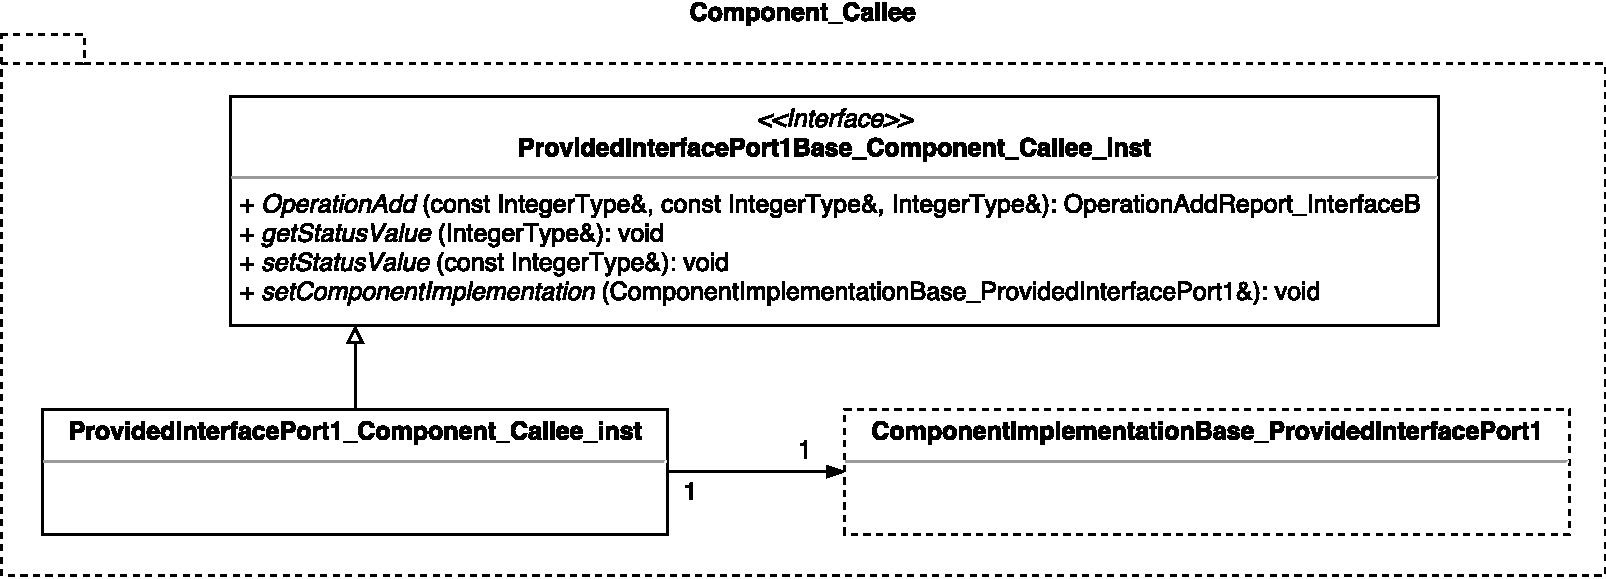
\includegraphics[width=1.0\textwidth]{ProvidedInterfacePort1UML.pdf}
	\caption{UML class diagram representation of \texttt{Provided\allowbreak Interface\allowbreak Port1\allowbreak\_Component\allowbreak\_Callee\allowbreak\_inst} for \texttt{Component\allowbreak\_Callee} in the example OBSW model}
	\label{fig: Provided interface port1 UML}
\end{figure}

\begin{figure}[h]
	\centering
	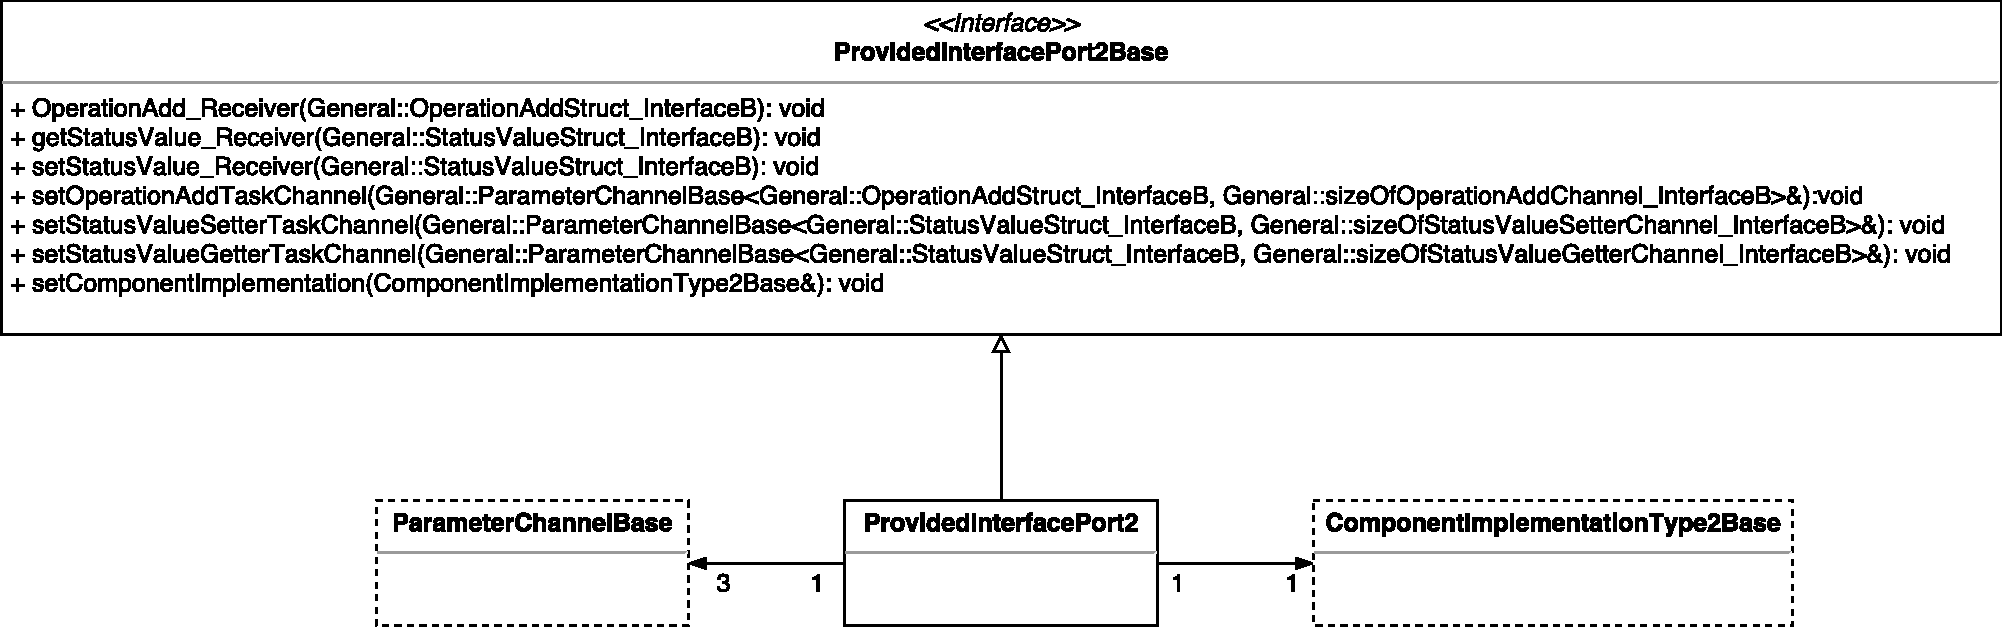
\includegraphics[width=1.0\textwidth]{ProvidedInterfacePort2UML.pdf}
	\caption{UML class diagram representation of \texttt{Provided\allowbreak Interface\allowbreak Port2\allowbreak\_Component\allowbreak\_Callee\allowbreak\_inst} for \texttt{Component\allowbreak\_Callee} in the example OBSW model}
	\label{fig: Provided interface port2 UML}
\end{figure}

\begin{figure}[h]
	\centering
	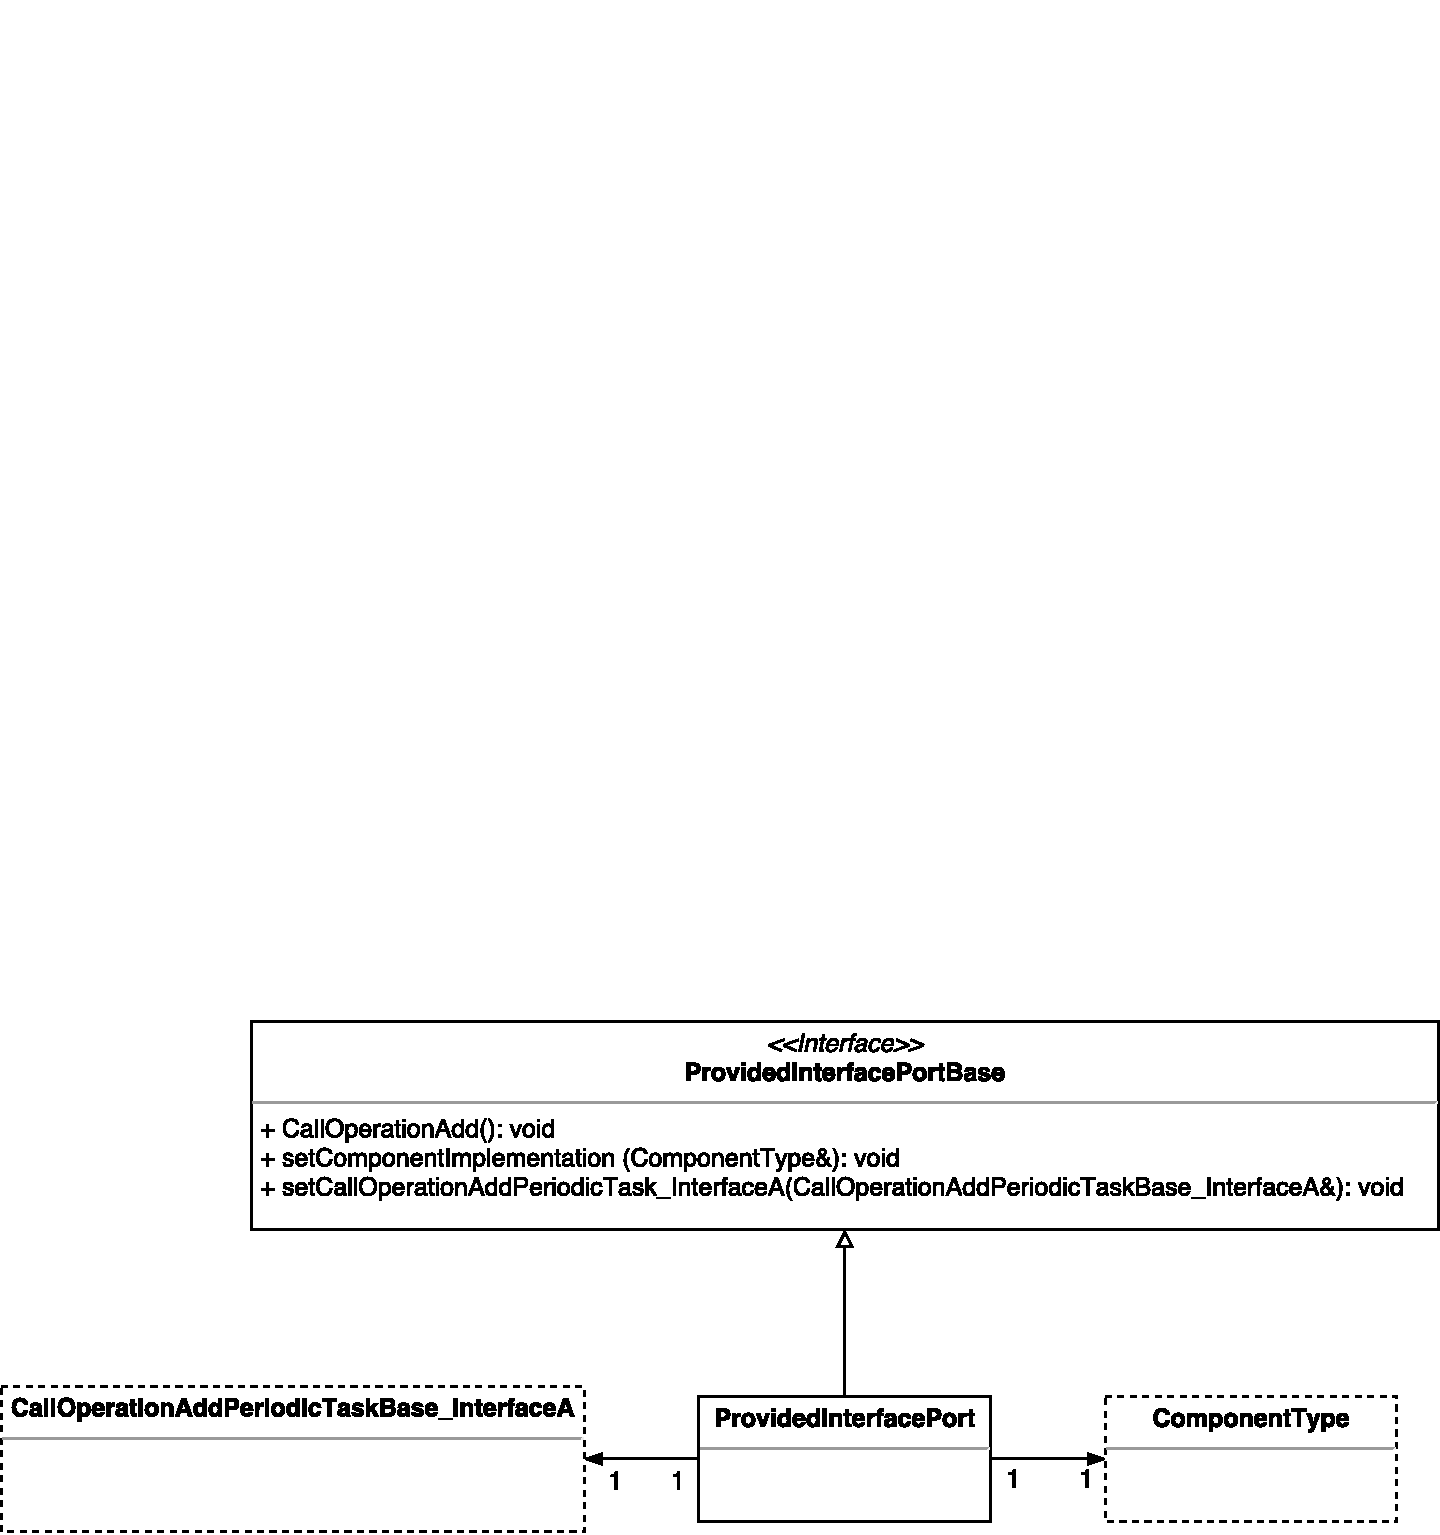
\includegraphics[width=1.0\textwidth]{ProvidedInterfacePortUML.pdf}
	\caption{UML class diagram representation of \texttt{Provided\allowbreak Interface\allowbreak Port\allowbreak\_Component\allowbreak\_Caller\allowbreak\_inst} for \texttt{Component\allowbreak\_Caller} in the example OBSW model}
	\label{fig: Provided interface port UML}
\end{figure}   

The concrete implementation for the above pure-virtual methods, in case the corresponding operation is requested to be released synchronously, consists of a simple call to the corresponding method in the referenced component implementation base class as shown in code excerpt in \cref{Listing: Provided interface port1 Impl}. If the non-functional property attached with release of the operation on the provided interface side is \texttt{Protected}, then the implementation also includes acquiring and releasing of semaphore associated with the operation as shown in code excerpt in \cref{Listing: Provided interface port1 Impl}. 

\begin{Listing}
\begin{lstlisting}[language=C++]
General::OperationAddReport ProvidedInterfacePort1_Component_Callee_inst::OperationAdd (const IntegerType& a,const IntegerType& b,IntegerType& c) {
	General::OperationAddReport_InterfaceB myReport;
	m_myComponent->lockOperationAdd_InterfaceB();
	myReport = m_myComponent->OperationAdd(a,b,c); //Simple method call
	m_myComponent->releaseOperationAdd_InterfaceB();
	return myReport;
}
\end{lstlisting}
\caption{Code excerpt from the generated code for operation \texttt{OperationAdd} access in \texttt{Provided\allowbreak Interface\allowbreak Port1\_\allowbreak Component\_\allowbreak Callee\_\allowbreak inst} which is called synchronously and has \texttt{Protected} as a non-functional property attached to it}
\label{Listing: Provided interface port1 Impl}
\end{Listing}

The concrete implementation for the above pure-virtual methods, in case the corresponding operation is requested to be released asynchronously, consist of pushing the data structure associated with the operation onto the corresponding task channel as shown in code excerpt in \cref{Listing: Provided interface port2 Impl} . A diagrammatic representation of the push that is required, is already shown in figures \cref{fig: Asynchronous sporadic}, \cref{fig: Asynchronous protected}, \cref{fig: Asynchronous bursty}, in the section which deals with the required code archetypes in the programming model for asynchronous release patterns.

\begin{Listing}
\begin{lstlisting}[language=C++]
void ProvidedInterfacePort2_Component_Callee_inst::OperationAdd_Receiver (General::OperationAddStruct_InterfaceB myStruct) {
	m_myOperationAddChannel->push(myStruct); //A push onto the task channel
}
\end{lstlisting}
\caption{Code excerpt from the generated code for operation \texttt{OperationAdd} access in \texttt{Provided\allowbreak Interface\allowbreak Port2\_\allowbreak Component\_\allowbreak Callee\_\allowbreak inst} which is called asynchronously}
\label{Listing: Provided interface port2 Impl}
\end{Listing}

The concrete implementation for the above pure-virtual methods, in case the corresponding operation is requested to be released with non-functional property as \texttt{cyclic}, then is a simple call to start the task using the reference to the task as shown in the code excerpt in \cref{Listing: Provided interface port Impl}.

\begin{Listing}
\begin{lstlisting}[language=C++]
void ProvidedInterfacePort_Component_Caller_inst::CallOperationAdd(void) {
	m_mycallOperationAddTask->startPeriodicTask(); //Method call to start the task
}
\end{lstlisting}
\caption{Code excerpt from the generated code for operation \texttt{CallOperationAdd} in \texttt{Provided\allowbreak Interface\allowbreak Port\_\allowbreak Component\_\allowbreak Caller\_\allowbreak inst} which has non-functional property set as \texttt{Cyclic}}
\label{Listing: Provided interface port Impl}
\end{Listing}

\textbf{For our example OBSW model}: The following classes as shown in \cref{fig: Provided interface port1 UML}, \cref{fig: Provided interface port2 UML}, \cref{fig: Provided interface port UML} are defined:
\begin{itemize}
\item \texttt{Provided\allowbreak Interface\allowbreak Port1\_\allowbreak Base\allowbreak Component\_\allowbreak Callee\_\allowbreak inst} abstract base class and its corresponding \texttt{Provided\allowbreak Interface\allowbreak Port1\_\allowbreak Component\_\allowbreak Callee\_\allowbreak inst} concrete implementation class
\item \texttt{Provided\allowbreak Interface\allowbreak Port2\_\allowbreak Base\allowbreak Component\_\allowbreak Callee\_\allowbreak inst} abstract base class and its corresponding \texttt{Provided\allowbreak Interface\allowbreak Port2\_\allowbreak Component\_\allowbreak Callee\_\allowbreak inst} concrete implementation class
\item \texttt{Provided\allowbreak Interface\allowbreak Port\_\allowbreak Base\allowbreak Component\_\allowbreak Caller\_\allowbreak inst} abstract base class and its corresponding \texttt{Provided\allowbreak Interface\allowbreak Port\_\allowbreak Component\_\allowbreak Caller\_\allowbreak inst} concrete implementation class 
\end{itemize} 

All the abstract base classes have pure virtual methods as per the general description given above and they have to be implemented in the corresponding concrete implementation classes. The concrete implementations are in line with the description as in the general case above.

\subsubsection{\textbf{Tasks from the Tasking framework}}
In the discussions about designing a programming model for OSRA in the \cref{chap: Progamming model}, it was clear that the threads of control might contain tasks from the Tasking framework. Each task is mapped to an abstract base class and a concrete implementation class in C++. A task would have instances of the required task inputs, task event as per the required threads of control explained in detail in the chapter on arriving at a programming model for OSRA.

Each task stores a reference to the base class of the component implementation in order to access the services implemented in the respective component implementations.  

\textbf{For our example OBSW model}: The following classes as shown in \cref{fig: Periodic task UML}, \cref{fig: Sporadic task UML}, \cref{fig: Status value getter setter task UML}, \cref{fig: Event receiver task UML} are defined:
\begin{itemize}
\item \texttt{CallOperationAdd\allowbreak Periodic\allowbreak TaskBase\_\allowbreak Provided\allowbreak Interface\allowbreak Slot} abstract base class and \texttt{Call\allowbreak OperationAdd\allowbreak Periodic\allowbreak Task\_\allowbreak Provided\allowbreak Interface\allowbreak Slot} concrete implementation class, in order to call operation \texttt{Call\allowbreak OperationAdd} in the \texttt{Provided\allowbreak Interface\allowbreak Slot} perioidically every 2s
\item \texttt{OperationAdd\allowbreak Sporadic\allowbreak TaskBase\allowbreak \_\allowbreak Provided\allowbreak Interface\allowbreak Slot2} abstract base class and a corresponding \texttt{Operation\allowbreak Add\allowbreak Sporadic\allowbreak Task\_\allowbreak Provided\allowbreak Interface\allowbreak Slot2} concrete implementation class, in order to call operation \texttt{Operation\allowbreak Add} in the \texttt{Provided\allowbreak Interface\allowbreak Slot2} sporadically with an MIAT of 2s
\item \texttt{StatusValue\allowbreak SetterTaskBase\allowbreak \_\allowbreak Provided\allowbreak Interface\allowbreak Slot2} abstract base class and a corresponding \texttt{Status\allowbreak Value\allowbreak Setter\allowbreak Task\allowbreak \_\allowbreak Provided\allowbreak Interface\allowbreak Slot2} concrete implementation class, in order to provide asynchronous access to the setter operation of the interface attribute \texttt{Status\allowbreak Value} in the \texttt{Provided\allowbreak Interface\allowbreak Slot2}
\item \texttt{StatusValue\allowbreak GetterTaskBase\allowbreak \_\allowbreak Provided\allowbreak Interface\allowbreak Slot2} abstract base class and a corresponding \texttt{Status\allowbreak Value\allowbreak Getter\allowbreak Task\allowbreak \_\allowbreak Provided\allowbreak Interface\allowbreak Slot2} concrete implementation class, in order to provide asynchronous access to the getter operation of the interface attribute \texttt{Status\allowbreak Value} in the \texttt{Provided\allowbreak Interface\allowbreak Slot2}
\item \texttt{Failure\allowbreak Event\allowbreak Receiver\allowbreak Task\allowbreak Base} abstract base class and a corresponding \texttt{Failure\allowbreak Event\allowbreak Receiver\allowbreak Task} concrete implementation class, for the reception of \texttt{Failure\allowbreak Event} which are emitted by the \texttt{Component\allowbreak\_Callee} asynchronously and to forward it to \texttt{Component\allowbreak\_Caller} 
\end{itemize} 

\begin{figure}[h]
	\centering
	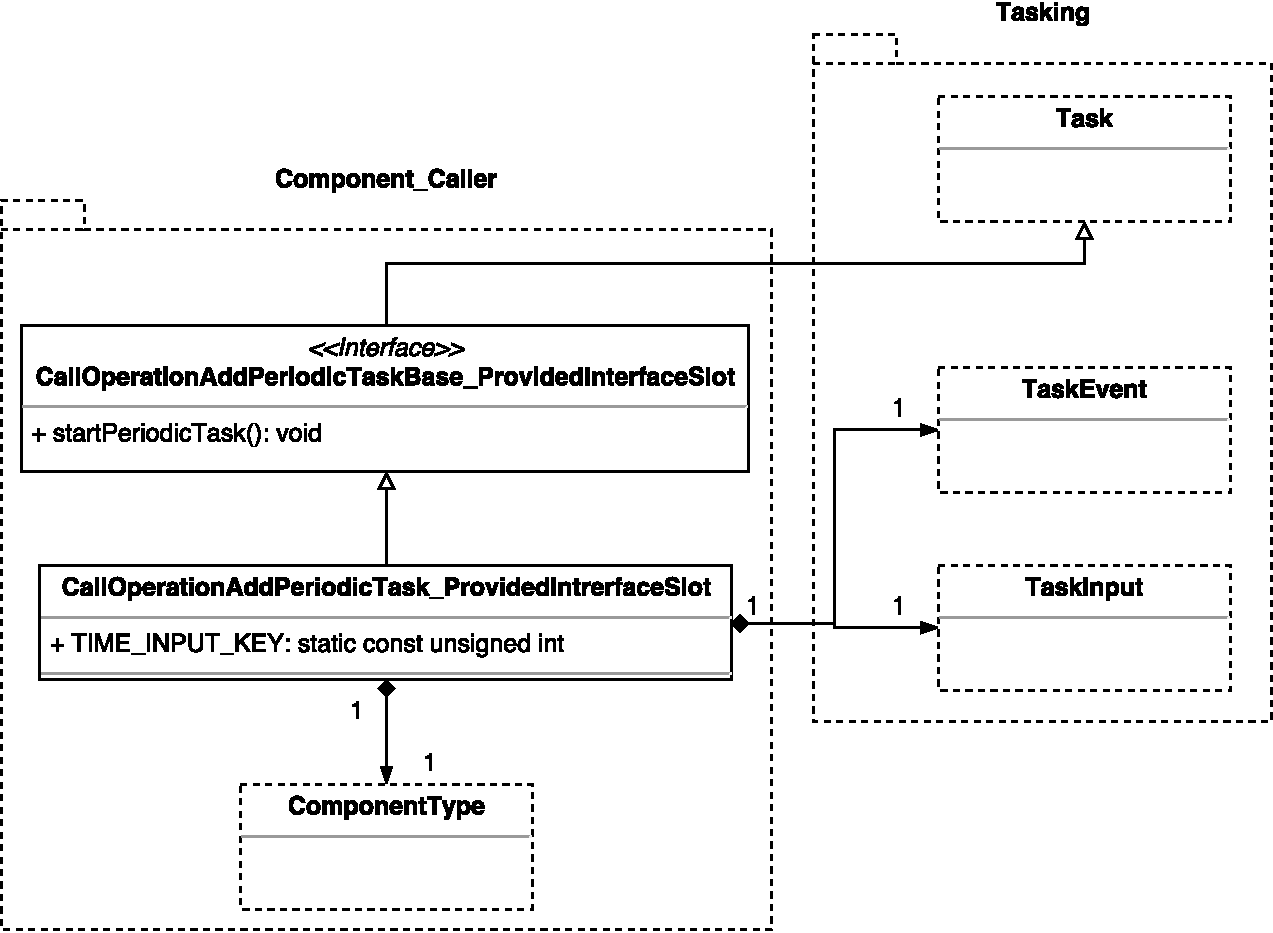
\includegraphics[width=0.8\textwidth]{PeriodicTaskUML.pdf}
	\caption{UML class diagram representation of the task required to call \texttt{CallOperationAdd} in \texttt{Provided\allowbreak Interface\allowbreak Port\allowbreak\_Component\allowbreak\_Caller\allowbreak\_inst} perioidcally with a period of 2s in the example OBSW model}
	\label{fig: Periodic task UML}
\end{figure}

\begin{figure}[h]
	\centering
	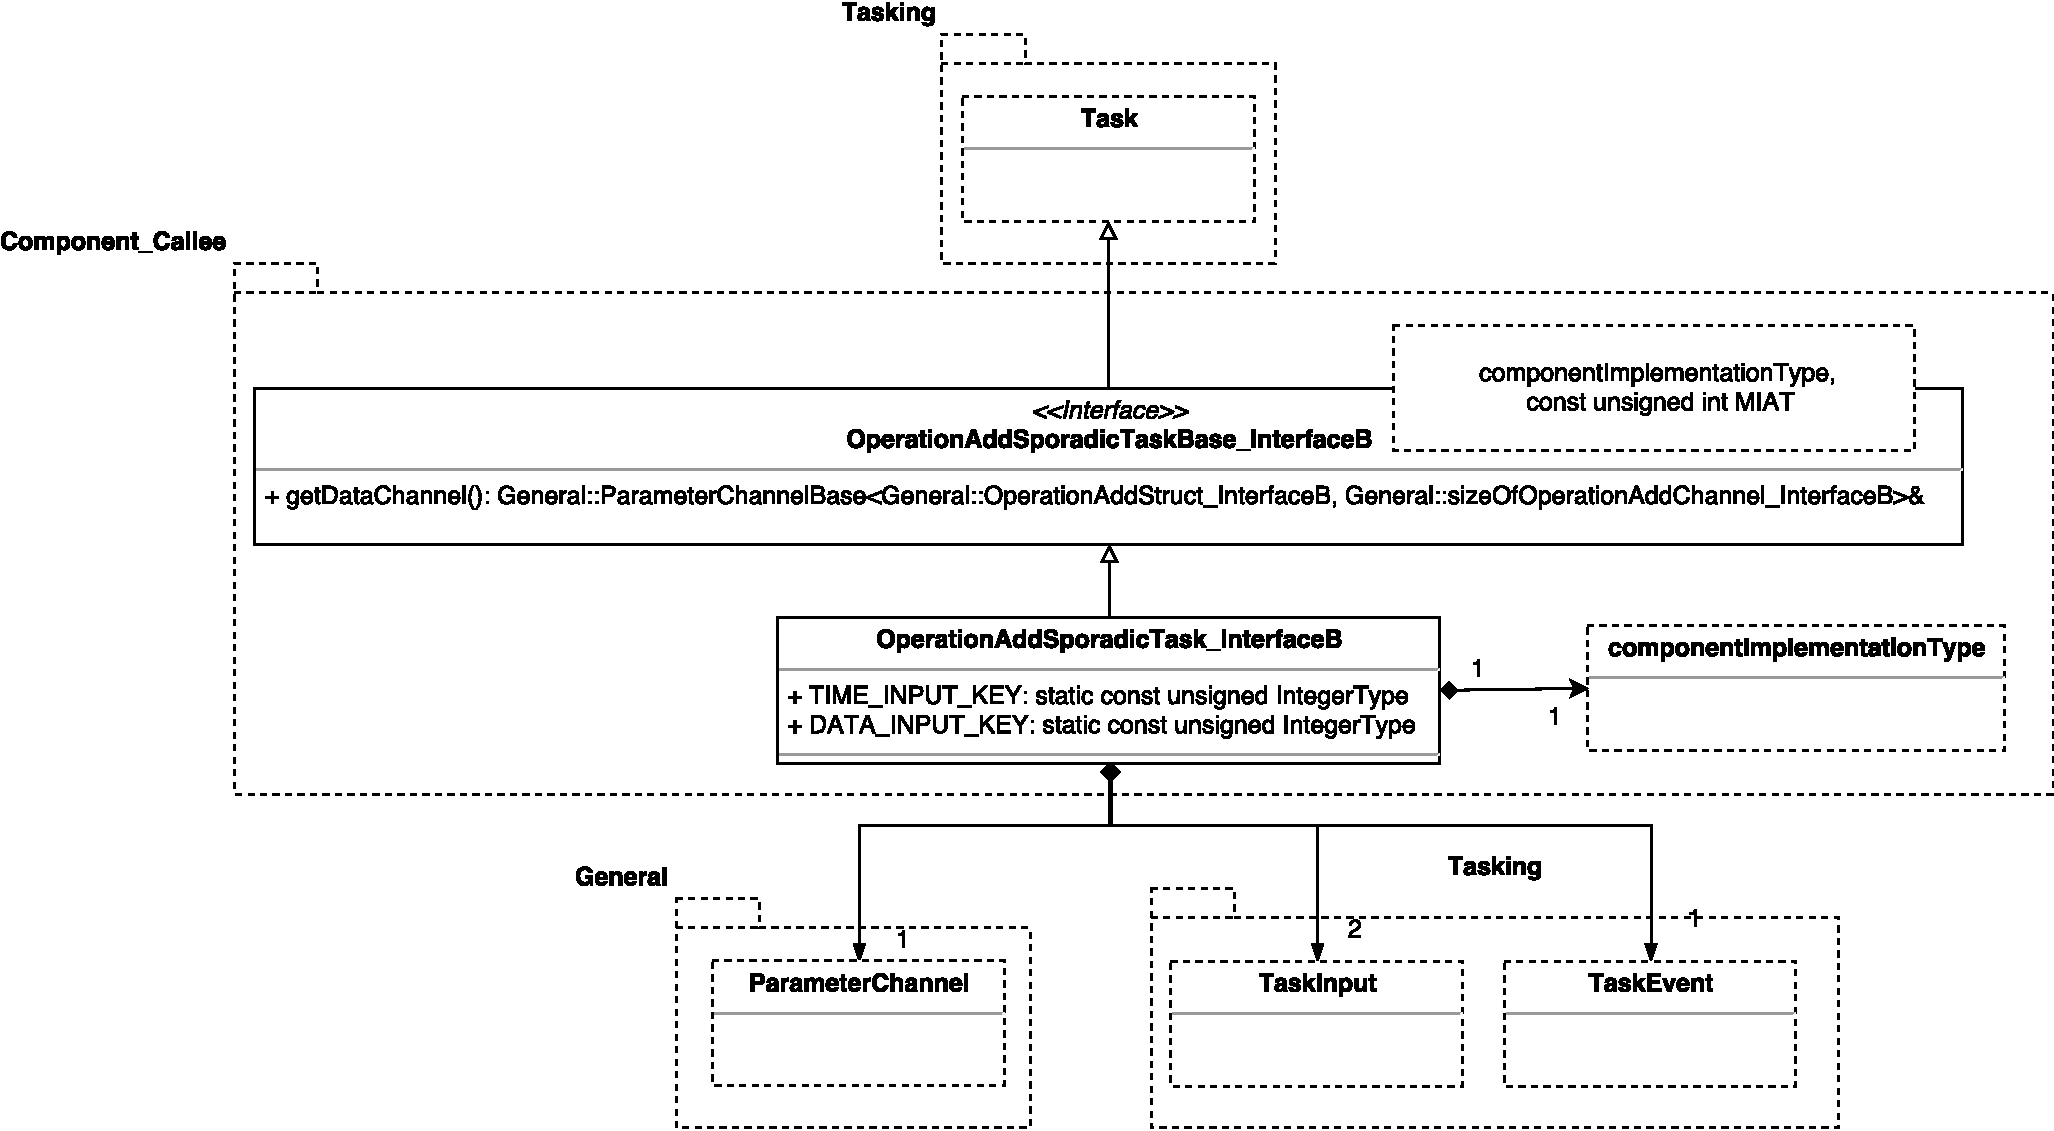
\includegraphics[width=1.0\textwidth]{SporadicTaskUML.pdf}
	\caption{UML class diagram representation of the task required to call \texttt{OperationAdd} in \texttt{Provided\allowbreak Interface\allowbreak Port2\allowbreak\_Component\allowbreak\_Callee\allowbreak\_inst} sporadically with a MIAT of 2s in the example OBSW model}
	\label{fig: Sporadic task UML}
\end{figure}

\begin{figure}[h]
	\centering
	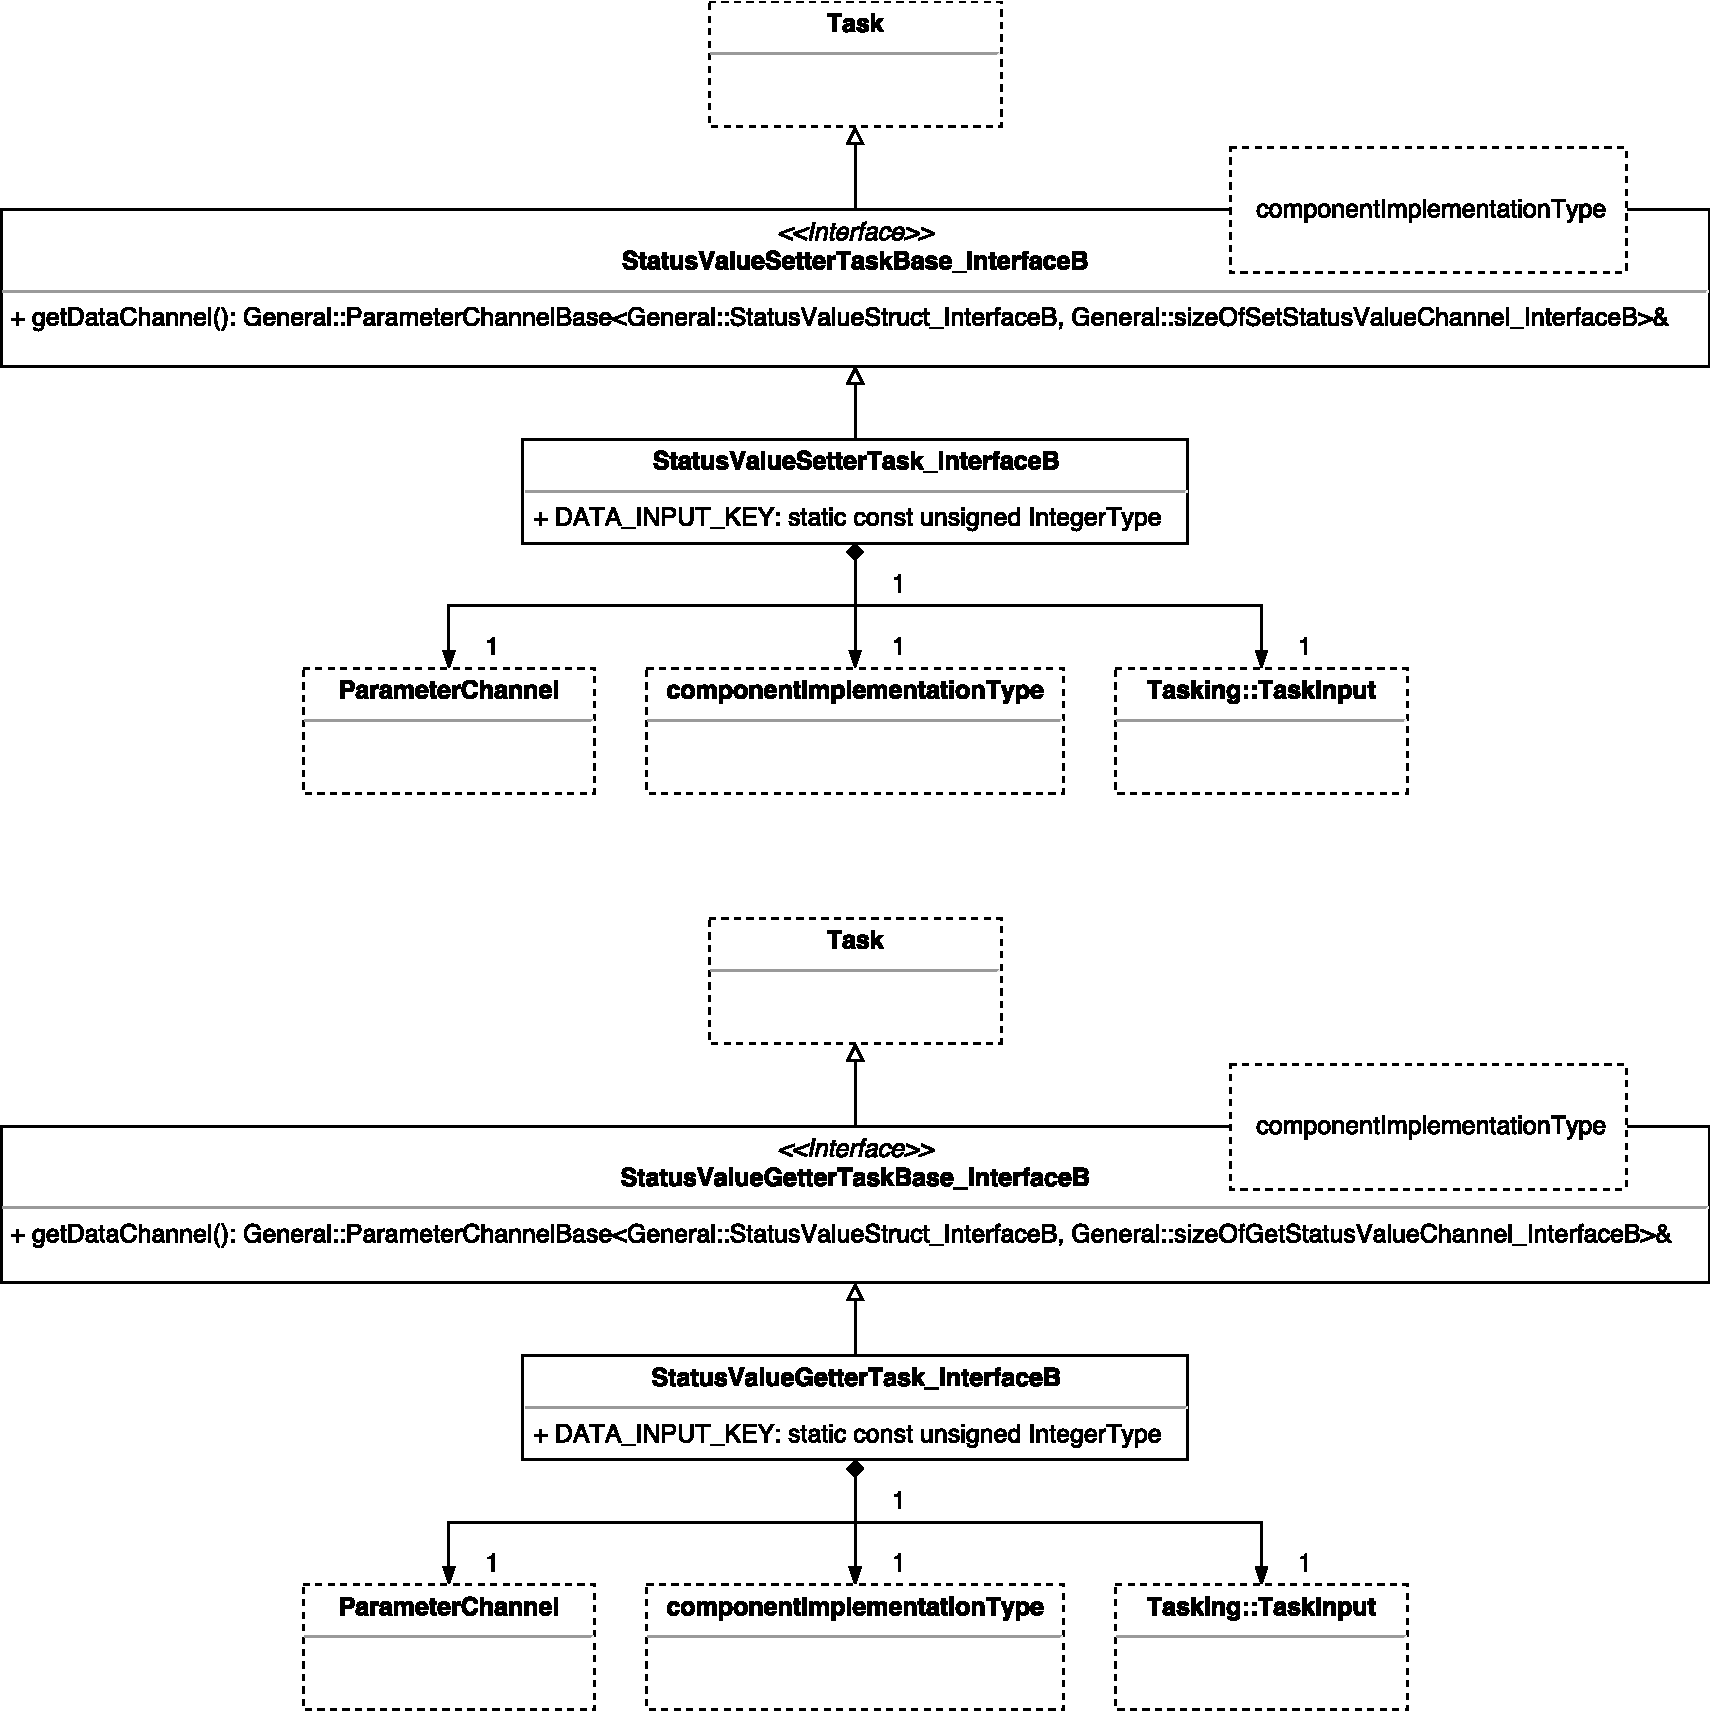
\includegraphics[width=1.0\textwidth]{SetterGetterTaskUML.pdf}
	\caption{UML class diagram representation of the tasks required to set and get the values of the interface attributes asynchronously in \texttt{Provided\allowbreak Interface\allowbreak Port2} in the example OBSW model}
	\label{fig: Status value getter setter task UML}
\end{figure}

\begin{figure}[h]
	\centering
	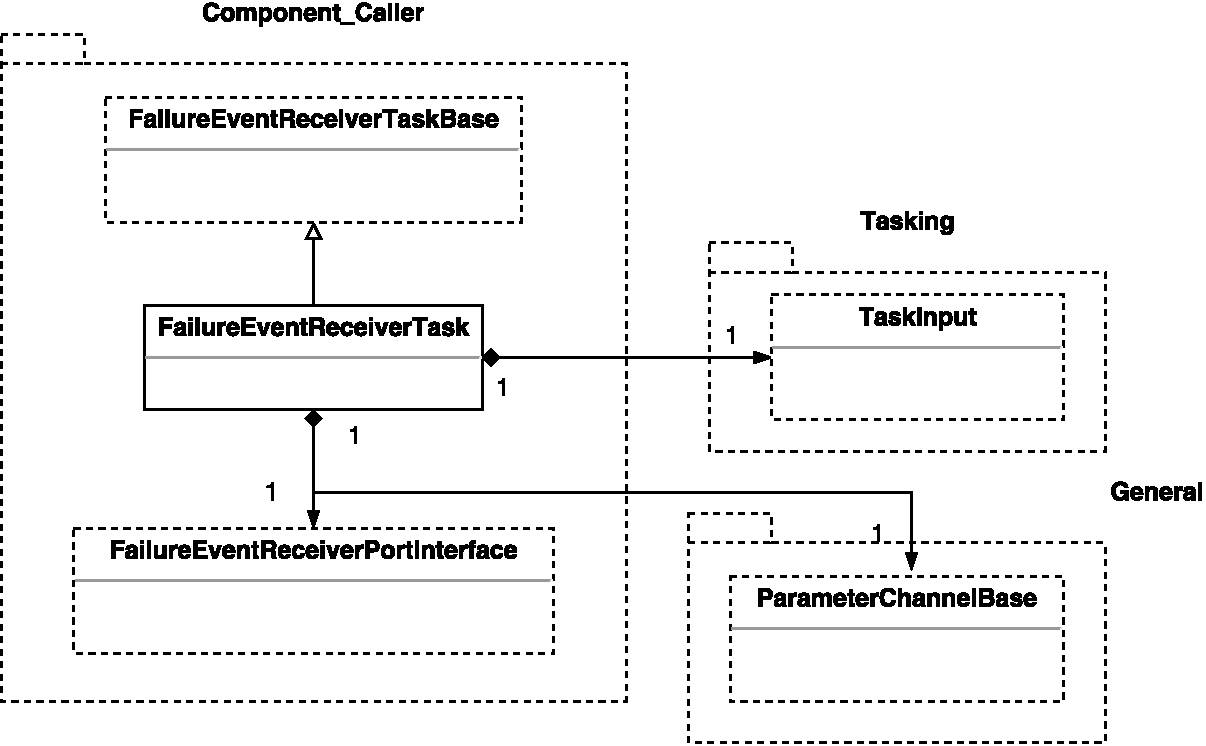
\includegraphics[width=0.8\textwidth]{FailureEventReceiverTaskUML.pdf}
	\caption{UML class diagram representation of the task required for the reception of the \texttt{Failure\allowbreak Event} in the example OBSW model}
	\label{fig: Event receiver task UML}
\end{figure}

\subsubsection{\textbf{Component containers}}
A container of a component can be mapped to a class in C++ as in \cite{EvoRAVCodeAr}. A component container consists of the following things:

\begin{itemize}
\item Instances of required interface ports
\item Instance of component implementation 
\item Instances of tasks which are necessary to handle services which are called asynchronously 
\item Instances of tasks which are necessary to receive asynchronous events
\item Instances of event emitter ports
\end{itemize}

A component container is also responsible for initializing the following:

\begin{itemize}
\item The instantiated component instance by providing references of the event emitter ports
\item The event emitter port by providing reference of the task channel to which the emitter port needs to push the information about the event
\item The provided interface ports by:
\begin{itemize}
\item Triggering the operations in the provided interface ports which have the desired non-function property set as \texttt{cyclic} 	
\item Providing reference of the component instance in order to access the service
\item Providing references of the different task channels they need to push the data structures associated with the operations onto, in order to handle the services which have the interaction kind specifies as \texttt{asynchronous} 
\end{itemize}
\item The instances of tasks with reference of component instance in order to schedule the execution of the services
\item The required interface ports by providing references of:
\begin{itemize}
\item The instantiated component instance, in order to initialize the data structures of the operations with correct function wrappers for call-back functions
\item The respective provided interface port each one of them is bound to 
\end{itemize}
\item The event receiver tasks with references of the component instance and the channels which needs to be associated with their respective task inputs      
\end{itemize}

\textbf{For our example OBSW model}: The following classes as shown in \cref{fig: Component container caller UML} and \cref{fig: Component container callee UML} are defined:

\begin{itemize}
\item \texttt{Container} in the namespace \texttt{Component\allowbreak\_Caller} which is the container for the component instance \texttt{Component\allowbreak\_Caller\allowbreak\_impl\allowbreak\_inst} and its provided and required interface slots
\item \texttt{Container} in the namespace \texttt{Component\allowbreak\_Callee} which is the container for the component instance \texttt{Component\allowbreak\_Callee\allowbreak\_impl\allowbreak\_inst} and its provided interface slots 
\end{itemize}

\begin{figure}[h]
	\centering
	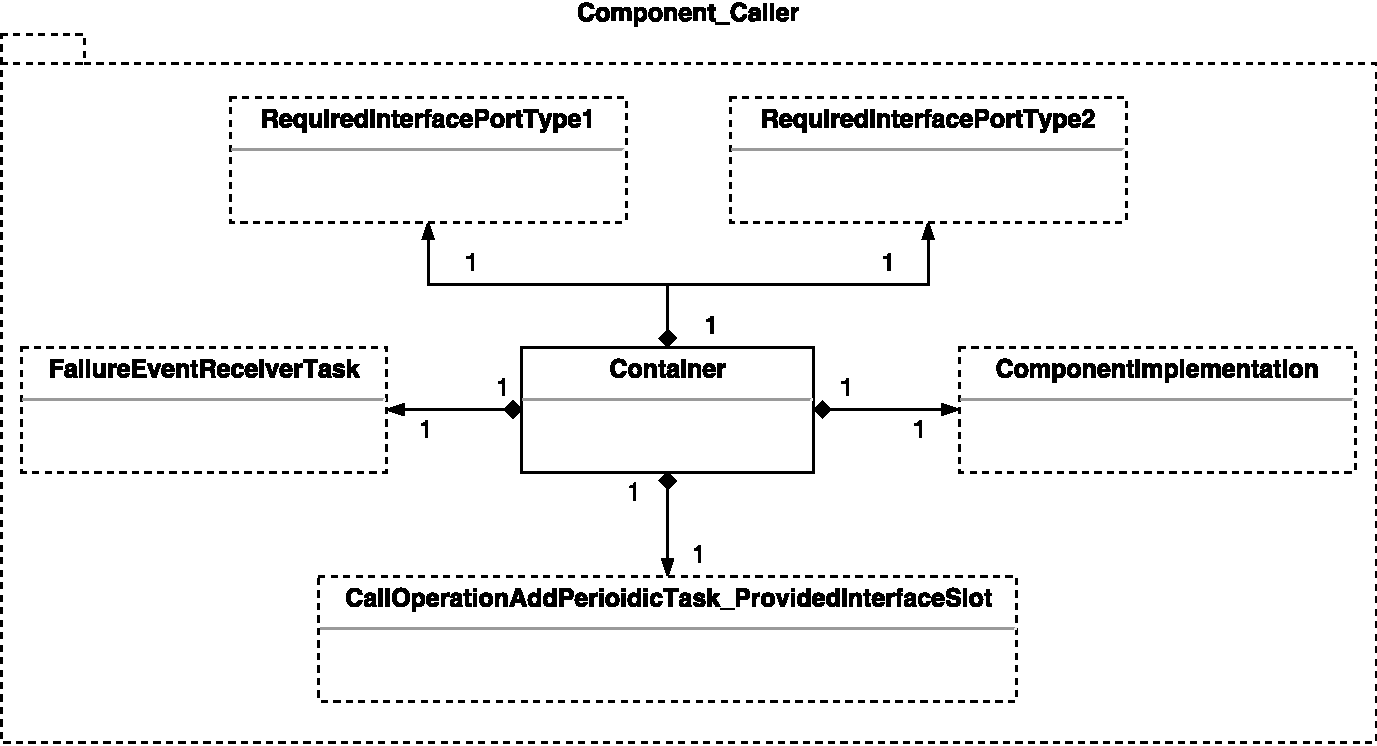
\includegraphics[width=0.8\textwidth]{ComponentContainerCallerUML.pdf}
	\caption{UML class diagram representation of the container for \texttt{Component\allowbreak \_Caller} in the example OBSW model}
	\label{fig: Component container caller UML}
\end{figure}

\begin{figure}[h]
	\centering
	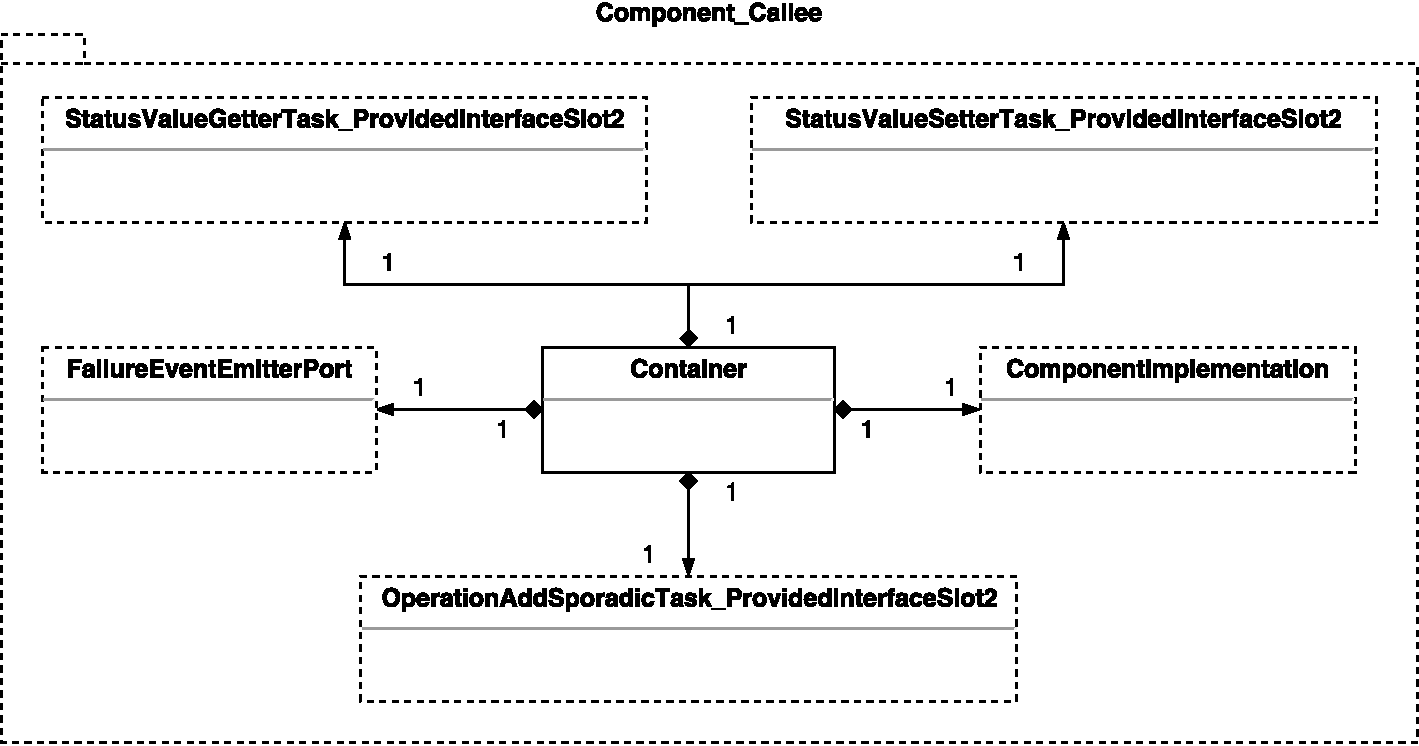
\includegraphics[width=0.8\textwidth]{ComponentContainerCalleeUML.pdf}
	\caption{UML class diagram representation of the container for \texttt{Component\allowbreak \_Callee} in the example OBSW model}
	\label{fig: Component container callee UML}
\end{figure}

Both the containers have instances of their respective different components as explained in the general case and as shown in \cref{fig: Component container caller UML} and \cref{fig: Component container callee UML}. They are responsible for the initialization of different components as explained in the above general description.  

\section{Code generation using Xtend}
\label{section: code generation}
The reference implementation of the OSRA component model consists in a set of .ecore metamodels \cite{SpecMetamodel}. Ecore is an implementation of the \ac{emof}, the meta-meta language by the OMG for the specification of meta-models \cite{SpecMetamodel}. The main advantage of using Ecore is the ready availability of graphical editors for the specification of metamodels and powerful support provided by the Eclipse Modeling Framework (EMF), which is a framework of the Eclipse development platform that permits to generate a code implementation of the metamodel entities, basic editors for the creation of models conforming to the metamodel under development \cite{SpecMetamodel}. 

It is an implementation decision in this Master thesis to use Xtend for the code generation. Xtend is a general purpose Java-like language that is completely operable with Java \cite{Xtend}\cite{XtendDoc}. Xtend has a more concise syntax than Java and provides powerful features such as type inference, extension methods, dispatch methods, an lambda expressions and the all important multiline template expressions, which are useful when writing code generators \cite{Xtend}\cite{XtendDoc}. Xtend also provides powerful features that make model visiting and traversing really easy, straightforward, and natural to read and maintain. 

Xtext is an eclipse framework for implementing programming languages and \ac{dsl} \cite{Xtend}. Xtext helps to implement languages quickly, and most of all, it covers all the aspects of a complete language infrastructure like parser, code generator etc. Xtext uses Google Guice, which is a dependency injection framework to create and call a code generator \cite{Xtend}. The dependency injection pattern basically allows to inject implementation objects into a class hierarchy in a consistent way \cite{InvOfCntrlurl}. The Xtext's generator support can be used in Xtend directly to build code generators for non-Xtext based models, such as the OBSW models constructed using the OSRA component model \cite{CodeGenEclXtend}. 

The tutorial in \cite{CodeGenNonXtext} is used as a base in this Master thesis to construct a code generator using Xtend for non-Xtext based models and also provide a UI integration for the code generator.

\section{Organizing the generated code}
\label{section: Code organization}
As explained in the previous sections, adopting separation of concerns even at the implementation level is one of the primary goals of this chapter and we have successfully achieved it in the discussions on software design for the infrastructural code in \cref{subsection: Software design approach}. 

To further emphasize on separation of concerns at the implementation level, it is necessary to properly separate the generated infrastructure code into a meaningful files and a suitable file structure helping the third party software supplier to separate the automatically generated code from the code that needs to be supplied. This is of prime importance for the third party software supplier to not accidentally lose the implementations in successive code generation cycles. 

The overall idea would be to:
\begin{itemize}
\item Generate two types of folders to clearly separate the infrastructural code entities, at the component type level from the infrastructural code entities at the component instance level. The number of folders at the component instance level, depends on the actual number of component instances.   
\begin{itemize}
\item The first folder type would hold C++ classes related to its component type, required interface ports, event emitter ports, event receiver ports in the sub-folder named as \texttt{AutogeneratedCode}. It also contains C++ classes related to component implementations and because it is the unit of sub-contract, it is placed in a separate sub-folder named as \texttt{UserCode}. The third-party software supplier can alter the code in this folder safely without the fear of the code being overwritten by successive code generation cycles. Care is taken in the code generator to generate the classes in these files only once  
\item The second folder type would hold the C++ classes related to its component instances, namely, provided interface ports, component containers in the sub-folder named as \texttt{AutogeneratedCode}. As already explained the component container class for a component instance would contain provided and required interface slots, component instance itself   
\end{itemize} 
\item The folder named as \texttt{Datatypes\allowbreak Interfaces\allowbreak EventsAnd\allowbreak Exceptions} would hold C++ classes related to the data types, exceptions, events, parameter channel and their corresponding parameter queues 
\end{itemize}

The folder structure for our running example is listed in \cref{chap: File structure}.
  



 

   

 


 
   



 


 
